\documentclass[12pt,oneside]{book}
\usepackage{times,mathptmx}
\usepackage[pdftex]{graphicx}
\usepackage{calc}
\usepackage{tabularx,ragged2e,booktabs,caption,subcaption}
\usepackage{array}
\newcolumntype{L}[1]{>{\raggedright\let\newline\\\arraybackslash\hspace{0pt}}m{#1}}
\newcolumntype{C}[1]{>{\centering\let\newline\\\arraybackslash\hspace{0pt}}m{#1}}
\newcolumntype{R}[1]{>{\raggedleft\let\newline\\\arraybackslash\hspace{0pt}}m{#1}}
\usepackage{multirow}
\usepackage{tocloft}
\usepackage{xcolor}
\usepackage{color,soul}
\usepackage{amsmath}
\definecolor{linknavy}{rgb}{0,0,0.50196}
\definecolor{linkred}{rgb}{1,0,0}
\definecolor{linkblue}{rgb}{0,0,1}
\usepackage{float}
\usepackage{graphpap}
\usepackage{rotating}
\usepackage{graphicx}
\usepackage{geometry}
\usepackage{relsize}
\usepackage{ltablex}
\usepackage{longtable}
\usepackage{lscape}
\usepackage{amssymb}
\usepackage{makeidx} % Create index at end of document
\usepackage[nottoc,notlof,notlot]{tocbibind} % Put the bibliography and index in the ToC
\usepackage{lastpage} % Automatic last page number reference.
\usepackage[T1]{fontenc}
\usepackage{enumerate}
\usepackage{upquote}
\usepackage{moreverb}
\usepackage{xfrac}
\usepackage{cite}
\usepackage{tikz}
% \usepackage{subfig}
% \usepackage{caption}
\usepackage[toc,page]{appendix}
\usepackage{notoccite}
\usepackage{colortbl}
\usepackage{titlesec}
\titleformat{\chapter}[hang] 
{\normalfont\huge\bfseries}{\chaptertitlename\ \thechapter}{1em}{} 
\titlespacing*{\chapter}{0pt}{-30pt}{20pt}

\newcommand{\nopart}{\expandafter\def\csname Parent-1\endcsname{}} % To fix table of contents in pdf.

\usepackage{siunitx}
\sisetup{
    detect-all = true,
    input-decimal-markers = {.},
    input-ignore = {,},
    inter-unit-product = \ensuremath{{}\cdot{}},
    multi-part-units = repeat,
    number-unit-product = \text{~},
    per-mode = fraction,
    separate-uncertainty = true,
}

\usepackage{listings}
\usepackage{textcomp}
\definecolor{lbcolor}{rgb}{0.96,0.96,0.96}

\usepackage[pdftex,
        colorlinks=true,
        urlcolor=linkblue,     % \href{...}{...} external (URL)
        citecolor=linkred,     % citation number colors
        linkcolor=linknavy,    % \ref{...} and \pageref{...}
        pdfproducer={pdflatex},
        pdfpagemode=UseNone,
        bookmarksopen=true,
        plainpages=false,
        verbose]{hyperref}

\setlength{\textwidth}{6.5in}
\setlength{\textheight}{9.0in}
\setlength{\topmargin}{0.in}
\setlength{\headheight}{0.pt}
\setlength{\headsep}{0.in}
\setlength{\parindent}{0.0in}
\setlength{\itemindent}{0.25in}
\setlength{\oddsidemargin}{0.0in}
\setlength{\evensidemargin}{0.0in}
% \setlength{\leftmargini}{\parindent} % Controls the indenting of the "bullets" in a list
\setlength{\cftsecnumwidth}{0.45in}
\setlength{\cftsubsecnumwidth}{0.5in}
\setlength{\cftfignumwidth}{0.45in}
\setlength{\cfttabnumwidth}{0.45in}
\setlength{\parskip}{1em}

\newcommand{\titlesigs}
{
\large
\flushright{UL Firefighter Safety Research Institute\\
{\em Stephen Kerber, Director} \\
\hspace{1in} \\
}
}

\newcommand{\headerB}[1]{
\flushleft{
\fontsize{28}{33.6}\selectfont
\bf{#1}
}
}

\newcommand{\headerC}[1]{
\vspace{.5in}
\flushright{\fontsize{14}{16.8}\selectfont
#1}
}

% \newcolumntype{L}{>{\centering\arraybackslash}m{4cm}}

\floatstyle{boxed}
\newfloat{notebox}{H}{lon}
\newfloat{warning}{H}{low}

\newenvironment{conditions}
  {\par\vspace{\abovedisplayskip}\noindent\begin{tabular}{>{$}l<{$} @{${}={}$} l}}
  {\end{tabular}\par\vspace{\belowdisplayskip}}


% Rename chapter headings
\renewcommand{\chaptername}{}
\renewcommand{\bibname}{References}

\usepackage{fancyhdr}
\pagestyle{fancy}
\lhead{}
\rhead{}
\chead{}
\renewcommand{\headrulewidth}{0pt}

\begin{document}
\pagenumbering{gobble}

\bibliographystyle{unsrt}
%\pagestyle{empty}

\begin{minipage}[t][9in][s]{6.25in}


\headerB{
Impact of Fire Attack Utilizing \\
Interior and Exterior Streams on\\ 
Firefighter Safety and Occupant \\
Survival: Water Mapping\\
}

\normalsize

\headerC{
{
\flushleft{
Craig Weinschenk \\
Keith Stakes \\
Robin Zevotek \\
\vspace{0.2in}
UL Firefighter Safety Research Institute \\
Columbia, MD 21045 \\
\vspace*{2\baselineskip}

}

\vfill

\flushright{


\includegraphics[width=2.in]{Figures/General/FSRI_GraphicShield} \\[.3in]
}
}
}

\end{minipage}

\newpage
\hspace{5in}
\newpage

\frontmatter

\begin{minipage}[t][9in][s]{6.25in}
\pagenumbering{gobble}


\headerB{
Impact of Fire Attack Utilizing \\
Interior and Exterior Streams on\\ 
Firefighter Safety and Occupant \\
Survival: Water Mapping\\
}

\headerC{
\flushleft{
Craig Weinschenk \\
Keith Stakes \\
Robin Zevotek \\
\vspace{0.2in}
{UL Firefighter Safety Research Institute \\
Columbia, MD 21045 \\}}

\flushleft{\today \\}
}


\vfill

\flushright{
\includegraphics[width=2in]{Figures/General/FSRI_GraphicShield}}

\titlesigs

\end{minipage}

\frontmatter

\pagestyle{plain}
\pagenumbering{roman}

\begin{minipage}[t][9in][s]{6.25in}

\flushleft{In no event shall UL be responsible to anyone for whatever use or non-use is made of the information contained in this Report and in no event shall UL, its employees, or its agents incur any obligation or liability for damages including, but not limited to, consequential damage arising out of or in connection  with the use or inability to use the information contained in this Report. Information conveyed by this Report applies only to the specimens actually involved in these tests. UL has not established a factory Follow-Up Service Program to determine the conformance of subsequently produced material, nor has any provision been made to apply any registered mark of UL to such material. The issuance of this Report in no way implies Listing, Classification or Recognition by UL and does not authorize the use of UL Listing, Classification or Recognition Marks or other reference to UL on or in connection with the product or system.
}

\vspace{3in}


\vfill

\hspace{1in}

\end{minipage}

\newpage

\chapter*{\centering Acknowledgments}
	
This work was funded through a grant from the Department of Homeland Security's Assistance to Firefighters Grant Program under the Fire Prevention and Safety Grants: Research and Development. Without this critical funding and support, this vital fire service research would not be possible.

\vspace*{\baselineskip}

\begin{center}
	
\includegraphics[width=0.28\textwidth]{Figures/General/DHS}
\end{center}

\clearpage

To assist the design and implementation of the experiments for the Fire Attack study, fire service experts were gathered from across the world with knowledge in fire suppression and the impact of interior and exterior fire streams. The individuals below provided direction for the project, assisting in planing the experiments, witnessing the testing, and developing concrete conclusions. Their tireless support and effort make this project relevant to the fire service across the world. 


\begin{table}[!ht]
	\centering
	\caption*{Fire Service Technical Panel}
	\begin{tabular}{ll}
		\toprule[1.5pt]
		Name & Fire Department \\ 
		\midrule
		Steve Brisebois  & Montreal Fire Department \\ 
		Matt Carrigan    & Montgomery County Fire and Rescue Service \\ 
		Tony Carroll     & Washington DC Fire Department \\ 
		Albert Castillo  & Houston Fire Department \\ 
		Chad Christensen & Los Angeles County Fire Department \\ 
		John Chubb       & Dublin Fire Brigade \\ 		 		  
		Danny Doyle      & Pittsburgh Fire Department \\ 
		Aaron Fields     & Seattle Fire Department \\ 
		Jason Floyd      & Las Cruces Fire Department \\ 
		John Gallagher   & Boston Fire Department \\ 
		Chad Green       & Anchorage Fire Department \\ 
		Kelly Hanink     & Eden Prairie Fire Department \\ 
		Samuel Hittle    & Wichita Fire Department \\ 
		Jacob Hoffman    & Toledo Fire/Rescue Department \\ 
		Josh Hummel      & Howard County Department of Fire and Rescue Services \\ 
		Jerry Knapp      & West Haverstraw (NY) Fire Department \\ 
		Dennis Legear    & Oakland Fire Department \\ 
		Hans Neiling     & Zuid Limburg Fire \\ 
		Nick Martin      & Columbia Fire Department \\ 
		Ray McCormack    & Fire Department of New York \\ 
		John McDonough   & New South Wales Fire Department \\ 
		Jordan Mohr      & Sedgwick County Fire District 1 \\ 
		Steve Pegram     & Goshen Township Fire and EMS \\ 
		\bottomrule[1.25pt]
	\end{tabular}
\end{table}

The authors would also like to acknowledge Adam Barowy and Greg Sutter of UL LLC for their assistance in conducting the water mapping experiments, specifically with the operation of the Actual Delivery Density apparatus.

\cleardoublepage
\phantomsection
\addcontentsline{toc}{chapter}{Contents}
\tableofcontents

\cleardoublepage
\phantomsection
\addcontentsline{toc}{chapter}{List of Figures}
\listoffigures

\cleardoublepage
\phantomsection
\addcontentsline{toc}{chapter}{List of Tables}
\listoftables

\chapter{List of Acronyms}

\begin{tabbing}
\hspace{1.5in} \= \\
ADD \> Actual Delivered Density \\
AFG \> Assistance to Firefighters Grant program  \\
ANOVA \> Analysis of Variation \\
DHS \> U.S Department of Homeland Security   \\   
FEMA \> Federal Emergency Management Agency  \\
NIST \> National Institute of Standards and Technology \\
SB \> Smooth Bore \\
SS \> Straight Stream \\
UL FSRI \> UL Firefighter Safety Research Institute \\
USFA \> United States Fire Administration  \\
\end{tabbing}

\newpage

\mainmatter

\chapter*{\centering Abstract}

As research continues into how fire department interventions affect fire dynamics in the modern fire environment; questions continue to arise on the impact and implications of interior versus exterior fire attack on both firefighter safety and occupant survivability. Previous research into various types of fire ground ventilation, flow paths, and exterior fire streams has provided the fire service with an increased understanding of fire dynamics. However in some instances, the information from the studies may not support current practices which have been based on experience. This gap between the research to date and the fire ground suppression experience has driven the need for further study. Therefore, research into the various methods of fire attack will allow a broader understanding of how firefighter interventions on the fire ground can impact the outcome of both life safety and property protection. 

This study will build upon the fire research conducted to date by analyzing how firefighting tactics, specifically different fire suppression tools and tactics, affect the thermal exposure and survivability of both firefighters and building occupants and affect fire behavior in structures. The purpose of this study is to improve firefighter safety, fireground tactics, and the knowledge of fire dynamics by providing the fire service with scientific information, developed from water flow and full-scale fire testing, in representative single family homes. The project will be comprised of 3 parts:

\begin{itemize}
	\setlength{\itemindent}{0.25in}
	\item Part I:  Water Distribution
	\item Part II: Air Entrainment
	\item Part III: Full-Scale Residential Fire Experiments
	\end{itemize}

This report details the results and analysis from the water distribution experiments. These tests were conducted without the presence of fire to gain a fundamental understanding of water flow into compartments. Each test was designed to quantify water distribution within a compartment by evaluating the differences caused by various application methods, hose stream types, nozzle movements, pressures/flow rates, and stream locations and elevation angles. 


\chapter{Background}

Recent fire service research has highlighted the importance of applying water to the fire as quickly as possible. This tactical consideration has highlighted a knowledge gap and increased the interest in better understanding the impact of water applied as part of an interior or exterior attack. Many variables exist in fire attack that impact firefighter effectiveness and victim survivability including stream placement, the time required to get water on the fire, stream type, stream movement, air entrainment, steam development, hot gas cooling and contraction, and position of flow paths. The most important firefighting tool for many years at structure fires has been their hoseline; however, many questions have arisen as more research shows the impact of ventilation, flow paths, and exterior fire streams. Whether a fire attack crew chooses to apply water as part of an interior attack or as part of an exterior or ``transitional attack," they need to know what impact their stream has on the fire environment ahead of them. This is difficult on the fire ground because visibility is commonly limited and therefore most experience and first-hand accounts are from behind the nozzle. This results in beliefs about conditions (e.g. temperature) ahead of the nozzle team and the impact of their tactics on victim survivability; but knowledge of the actual impact has yet been researched. Additionally, when the fire is ultimately suppressed, there is no assurance the attack was conducted in the most effective, efficient, and safe manner even if the experience gained suggests that it was. Fire service adages such as ``don't put water on smoke,'' ``you will steam the victims,'' and ``fog nozzles always disrupt the thermal layer'' have been passed on from generation to generation with little context or substantiation. Without the context, these concepts get treated like rules and can severely limit firefighters understanding of fire suppression.

Current fire training curriculum defines 3 fire attack methods: direct attack, indirect attack, and combination attack. Direct attack involves the discharge of water directly onto the burning fuel. Indirect attack involves directing the stream toward the ceiling of a compartment in order to generate a large amount of steam in order to cool the compartment. Converting the water to steam displaces oxygen, absorbs the heat of the fire and cools the hot gas layer sufficiently for firefighters to safely enter and make a direct attack. Combination attack extinguishes a fire by using both a direct and indirect attack. Another technique to safely approach a fire that cannot be reached with a direct attack is gas cooling. Gas cooling provides a buffer zone around the attack team but the larger the compartment, the less the impact on cooling the hot gas layer. Gas cooling must be a continuous process while advancing toward a shielded fire. Techniques for effective gas cooling and the upper limit of the volume where gas cooling is effective is not well known.  

Fire suppression effectiveness and firefighter safety are not achieved by water flow rate alone, but by appropriate use of a given flow rate under specific fire ground conditions. A flow rate must meet the critical flow rate to extinguish a fire depending on the heat release rate and should be higher to reduce the time to extinguishment. Drastically exceeding the critical flow rate has less known impact on time to extinguishment but has a significant impact on the total amount of water used. To-date, there is little data to connect the critical flow rate to firefighter safety. However, it has been estimated that only 5 to 10 percent of water applied during fire attack contributes to extinguishment. It is difficult for firefighters to realize the the efficiency of various hose stream techniques due to poor visibility on the fireground. However, by developing data in realistic structures, fuel sources, and fire scenarios, important inferences may be developed relative to different hose stream techniques, and use of water.

\subsubsection*{Hose Streams} %Only created paragraph so we have a heading to move this section around
Hose streams, often titled ``Fire Streams'' in traditional fire service training manuals are defined many was however all with the same general theme. A hose stream is the pattern of water which exits a nozzle, supplied via a fire hose. The two main fire service nozzles are a combination nozzle and smooth bore nozzle. 

\chapter{Objectives}

The purpose of this part to the overall study was to provide scientific knowledge on the variation of water flow rate per square foot (water flux) during interior and exterior fire attack. This was accomplished with the completion of the following objectives:

\begin{itemize}
	\setlength{\itemindent}{0.25in}
	\item Adapt measurement apparatus common to sprinkler testing for use in hose stream flow quantification.
	\item Quantify repeatability and uncertainty in apparatus.
	\item Measure water flux data distributions in typical residential compartment for common fire service hose stream configurations.
	\item Quantify similarities and differences of water flux distributions over the range of test variables.
	\item Develop and disseminate knowledge of hose streams applied during typical interior and exterior fire attack.
	\end{itemize}


\chapter{Water Distribution Experiments}

The goal of the water distribution experiments was to quantify the impact that changing a nozzle, changing flow pressure, or changing flow position had on water dispersion within a compartment. Eighty-four water flow tests were conducted at the UL Large Fire Laboratory in Northbrook, IL in a purpose built compartment with an attached hallway and movable staircase. Water flow patterns were determined by collecting the water in 48 discrete collection bins.

\section{Experimental Configuration}

\subsection{Test Apparatus}
\label{ADD_discussion}
The main portion of the test compartment had interior (finished) dimensions of 17~ft 4~in. by 11~ft 4~in with an 8~ft ceiling. To account for water collection apparatus the entire compartment was 7~ft 10 7/8~in above the floor of the lab floor (see Figure~\ref{fig:Water_Distribution_Test_Structure_and_ADD_Apparatus}). The overall size of the compartment was designed to reflect that of one found in a typical resident structure but was also bound by the dimensions of the water collection apparatus (Section~\ref{sec:add_instrumentation}). The compartment was wood frame construction with 2~in. by 4~in. studs and track set to 16~in. centers with a interior height measuring 8~ft 1 1/8~in. rough. The walls and ceiling were lined with 1/2~in. durarock cement board atop 1/2~in. plywood. The ceiling joists were 2~in. by 6~in. set to 16~in. on center.

\begin{figure}[!ht]
	\centering
	\includegraphics[width=.8\columnwidth]{Figures/Water_Distribution/Building.jpg}
	\caption[Water Distribution Test Structure and ADD Apparatus]{Water Distribution Test Structure and ADD Apparatus.}
	\label{fig:Water_Distribution_Test_Structure_and_ADD_Apparatus}
\end{figure}

The compartment featured two openings; one doorway measuring 3~ft by 6~ft 8~in. which opened to the interior hallway, and one window measuring 2~ft by 4~ft which opened to the exterior of the compartment. A movable staircase and landing was constructed to provide access to either the interior hallway of the compartment or provide a simulation of a first floor exterior attack. The hallway was 6~ft by 8~ft and the stairway landing was 4~ft by 6~ft 8~in. Detailed dimension drawings of the compartment are included in Figures~\ref{fig:ADD_Top_View} and \ref{fig:ADD_Side_View}

\begin{figure}[!ht]
	\centering
	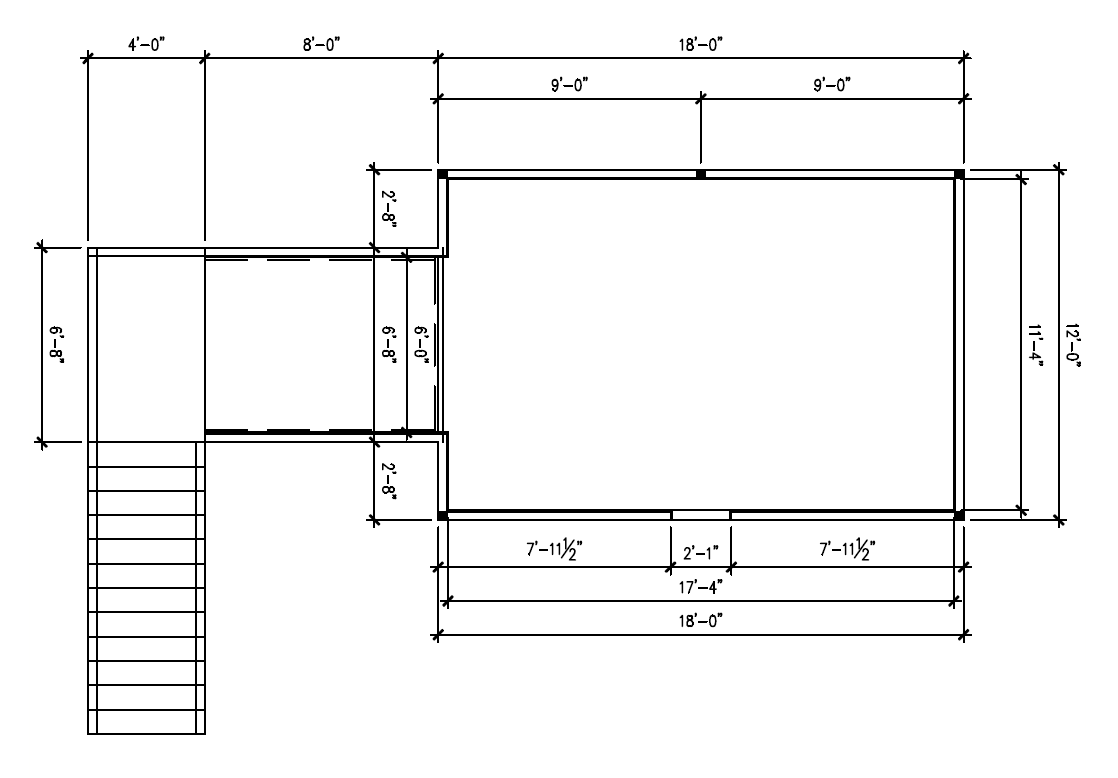
\includegraphics[width=\columnwidth]{Figures/Water_Distribution/ADDtopviewprint}
	\caption[ADD Plan View]{ADD Plan View.}
	\label{fig:ADD_Top_View}
\end{figure}

\begin{figure}[!ht]
	\centering
	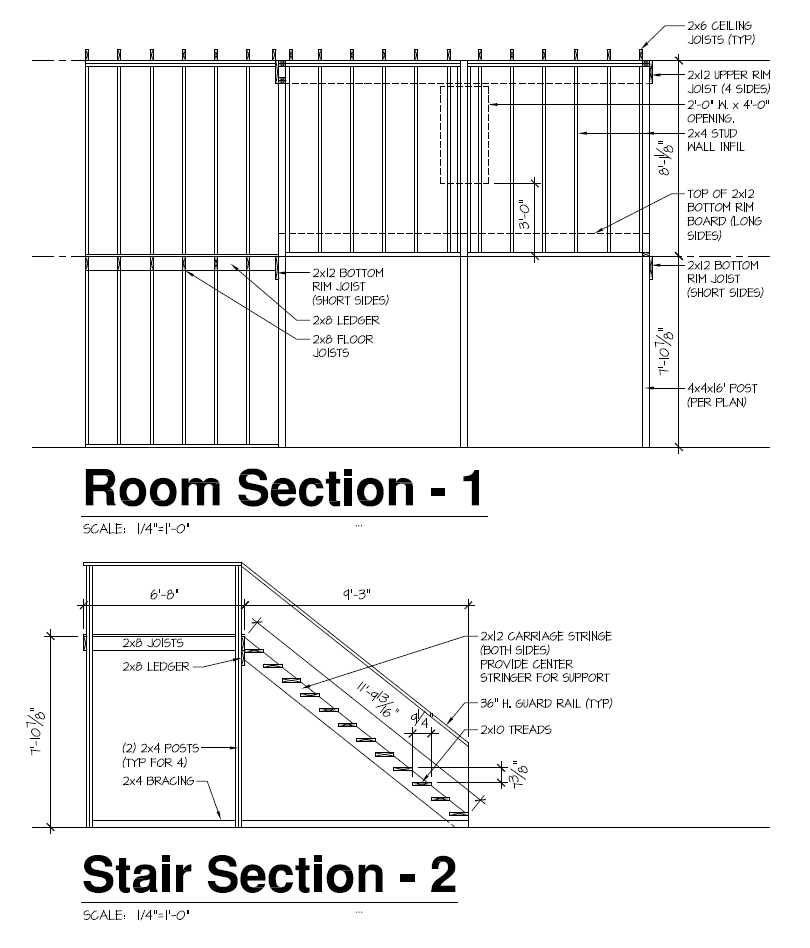
\includegraphics[width=\columnwidth]{Figures/Water_Distribution/ADDsideviewprint}
	\caption[ADD Side View]{ADD Section View.}
	\label{fig:ADD_Side_View}
\end{figure}

\clearpage

A unique feature of this compartment was that there was no floor constructed. The test compartment instead sat directly over 48, 20~in by 20~in stainless steel collection bins. Instead of water accumulating on the floor, in would flow into the distinct collection bins to determine an accumulation rate. Potential gaps between the collection bins were covered by flashing which was folded to divert the water evenly in each bin, to best ensure adequate distribution results. The gaps between the outer collection bins and the walls of the structure were also covered with flashing to ensure all water directed into the structure was collected in the appropriate bins. The interior layout of the floor bins and use of flashing can be seen in Figure \ref{fig:ADD_Flashing}. 

\begin{figure}[!ht]
	\centering
	\includegraphics[width=.7\columnwidth]{Figures/Water_Distribution/floor3.jpg}
	\caption{Layout of Structure Floor with 48 Collection Bins and Connected Flashing}
	\label{fig:ADD_Flashing}
\end{figure}

\subsection{Instrumentation and Uncertainty}
\label{sec:add_instrumentation}

To measure the water distribution throughout the compartment, a fire sprinkler spray density measurement instrument known as the Actual Delivered Density (ADD) apparatus was used~\cite{Schwille2005}. This device was connected to the 48 collection bins that comprised the floor of the test structure. The ADD apparatus is comprised of one main array and two satellite arrays of heavy steel framework. The main array consists of 32 water barrels and water pan collection assemblies while each satellite array contains 8 barrels and collection assemblies, see Figure~\ref{fig:ADD_Collection_Assembly}. All barrels are of 30-gallon capacity and are connected by a 2~in. diameter hose to a 20~in. by 20~in. inverted square pyramid shaped stainless steel water collection pan above. In total, there are 48 total collection pans/barrels. Differential pressure transducers connect to the bottom of each water collection barrel via flexible tubing. The water level in a given barrel is determined by the head pressure measured by the transducer. The water collection rate is calculated based the change in head pressure over time. As Figure \ref{fig:Bin Numbers and Locations} shows, collection assemblies were arranged into 2~$\times$~2 arrays. Each collection barrel is uniquely numbered so that water flow data can be mapped to specific position. The barrels are connected to a pneumatic drain valve which could be actuated to drain each barrel at the conclusion of an experiment. 

\begin{figure}[!ht]
	\centering
	\begin{tabular}{cc}
		\includegraphics[height = .3\columnwidth]{Figures/Water_Distribution/ADD2.jpg} &
		\includegraphics[height = .3\columnwidth]{Figures/Water_Distribution/ADDbottom3.jpg} \\
	\end{tabular}
	\caption[ADD Collection Barrels and Pans]{ADD Collection Barrels (left) and ADD Collection Pans (right).}
	\label{fig:ADD_Collection_Assembly}
\end{figure}

\begin{figure}[!ht]
	\centering
	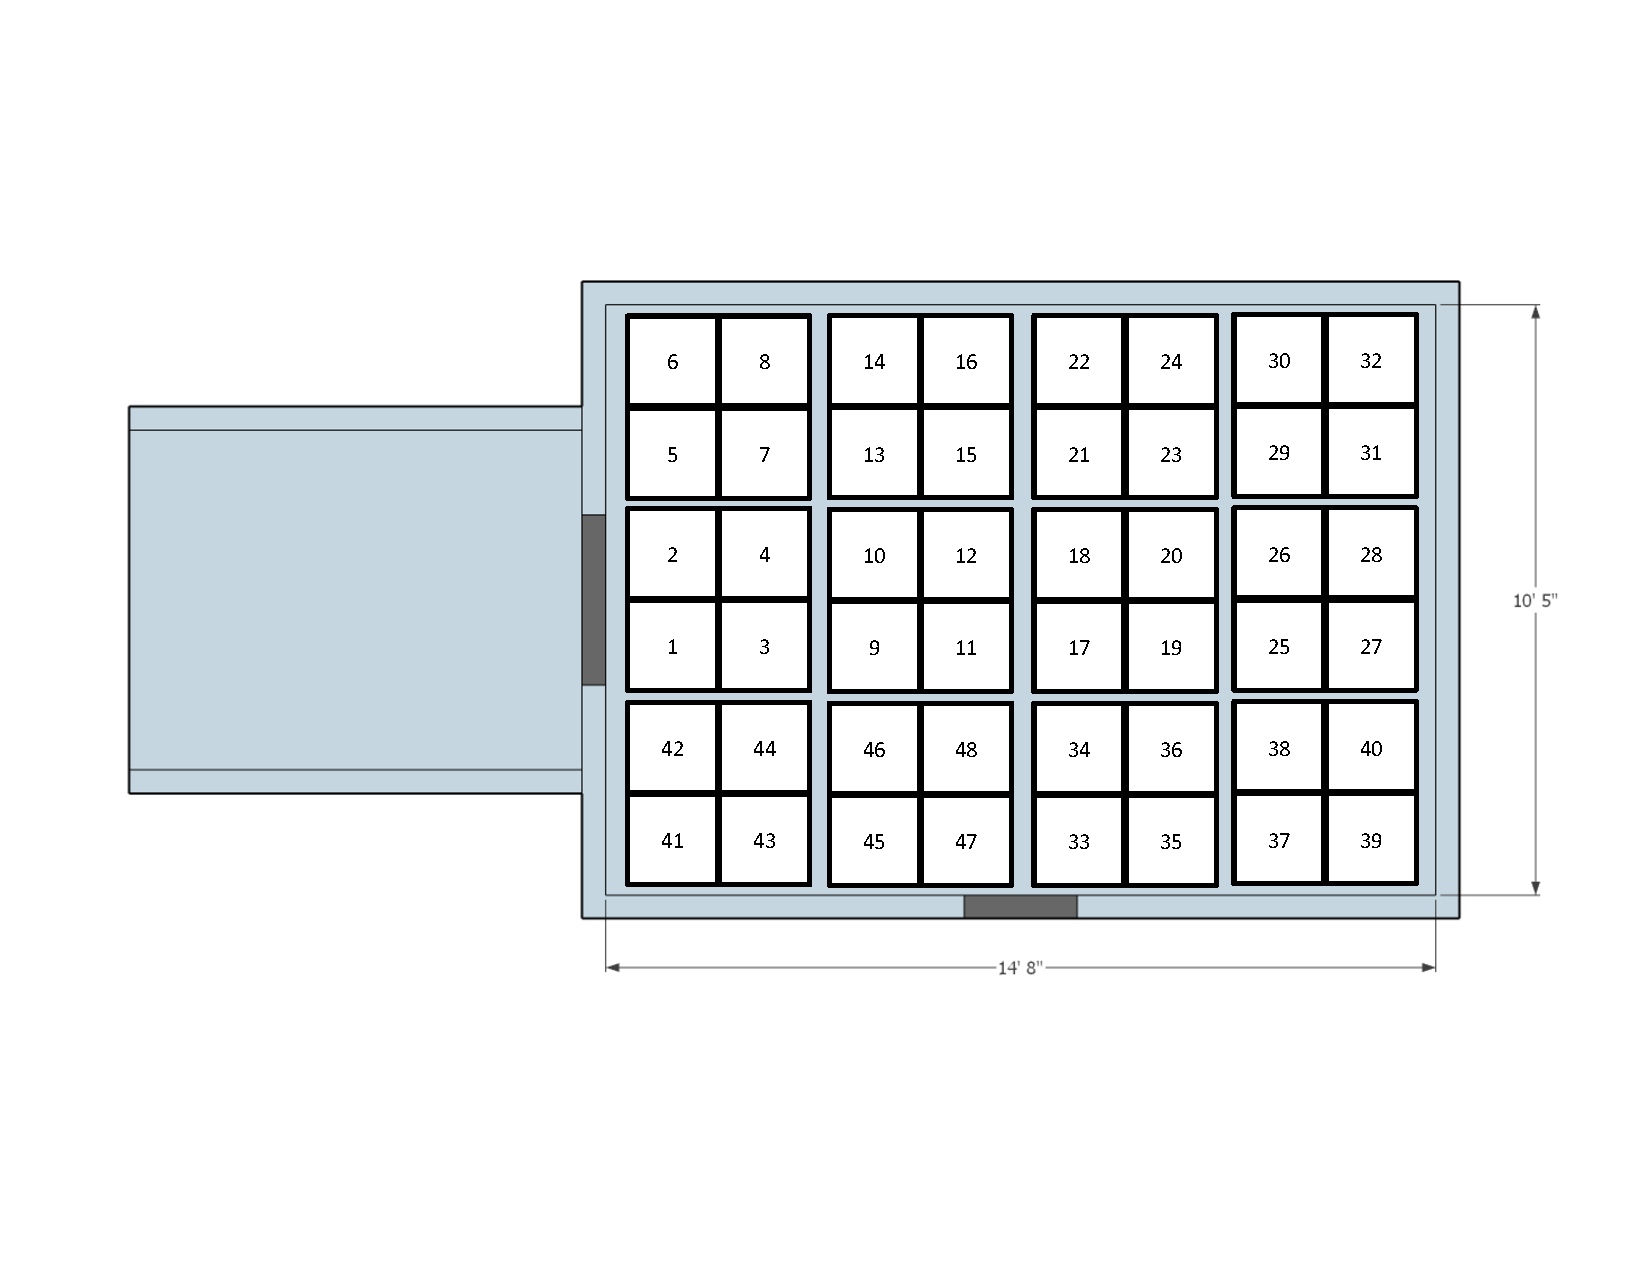
\includegraphics[width=\columnwidth]{Figures/Water_Distribution/Bin_Numbers_NoDimensions}
	\caption[ADD Bin Numbers and Locations]{ADD Bin Numbers and Locations}
	\label{fig:Bin Numbers and Locations}
\end{figure}

Prior to testing, data was collected to estimate the uncertainty associated with the water distribution measurements performed using the ADD apparatus. Each water collection assembly was filled to capacity while recording pressure transducer measurements as well as data from a calibrated turbine flowmeter (with less than 1~\% measurement uncertainty). Although the design of each water collection assembly is the same, the measurement performance across the entire apparatus varied. Overall, the 48 water collection assemblies reported an average accuracy of $\pm$ 2.4~gallons. This represents an uncertainty in total volume of $\pm$ 8~\% at full scale (30~gal).

\subsection{Experimental Equipment}

To ensure the data collected were applicable to the majority of the fire service, a representative set of nozzles types, specified flows/pressures, and hose sizes were used which are shown in Table~\ref{tab:nozzles_used_detail}.

\begin{table}[!ht]
\centering
\caption{Primary Equipment Configurations}
\label{tab:nozzles_used_detail}
\begin{tabular}{llccc}
\toprule[1.5pt]
Line Size & Nozzle Type & Tip (in) & Nozzle Pressure (psi) & Approximate Flow Rate (gpm) \\ 
\midrule
1 3/4 in. & Smooth Bore          & 1      & 50 & 210 \\
          & Smooth Bore          & 15/16  & 50 & 180 \\
          & Smooth Bore          & 7/8    & 50 & 150 \\
          & Combination          &        & 100 & 100 \\
          & Combination          &        & 100 & 150 \\
          & Combination          &        & 75 & 150 \\
          & Combination          &        & 50 & 150 \\ \midrule
2 1/2 in. & Smooth Bore          & 1 1/4  & 50 & 260 \\
          & Combination          &        & 100 & 250 \\
\bottomrule[1.25pt]
\end{tabular}
\end{table}

\section{Experiments Conducted}

The water distribution experiments consisted of 84 experiments with configuration variables of flow position, interior or exterior, nozzle type, pressure at the nozzle, stream angle and stream pattern. In each experiment, water flowed for approximately 1~min. in duration. If a barrel overflowed, there would be an inability to determine the correct distribution of water flow, therefore the duration was dictated by the size of the collection barrels in the ADD apparatus. Each collection barrel was a total of 30~gallons.  At the start of each test, there was an initial amount of water in the bottom of the barrel to ensure the sensors were able to record the water received during the testing. The total water in each barrel was determined by subtracting the initial water volume in each barrel from the final value. 

\subsection{Interior Experiments}
\label{int_tests}
The interior experiments were designed to simulate a fire on the same floor as the attack crew. Suppression operations were conducted from the doorway adjoining the hallway to the test compartment. At this location, hose stream type, nozzle direction, and nozzle movement were varied and the water distribution within the compartment was measured. The three nozzle directions, max angle ceiling, mid ceiling, and at wall are shown in Figure \ref{fig:Nozzle_Direction_Interior_Attack} and were set from a fixed nozzle location. The max angle ceiling position was defined to be the steepest angle the nozzle could be without the stream being impacted by the soffit of the doorway. The mid ceiling position set the stream to hit the middle of the ceiling along the 14~ft 8~in. dimension. The third position, the wall position, was defined to have the stream hit the vertical midpoint of the wall adjacent to the doorway. Table~\ref{tab:Interior_Fire_Attack_Distribution_Experiments} lists the interior experiments conducted.

\begin{figure}[!ht]
	\centering
	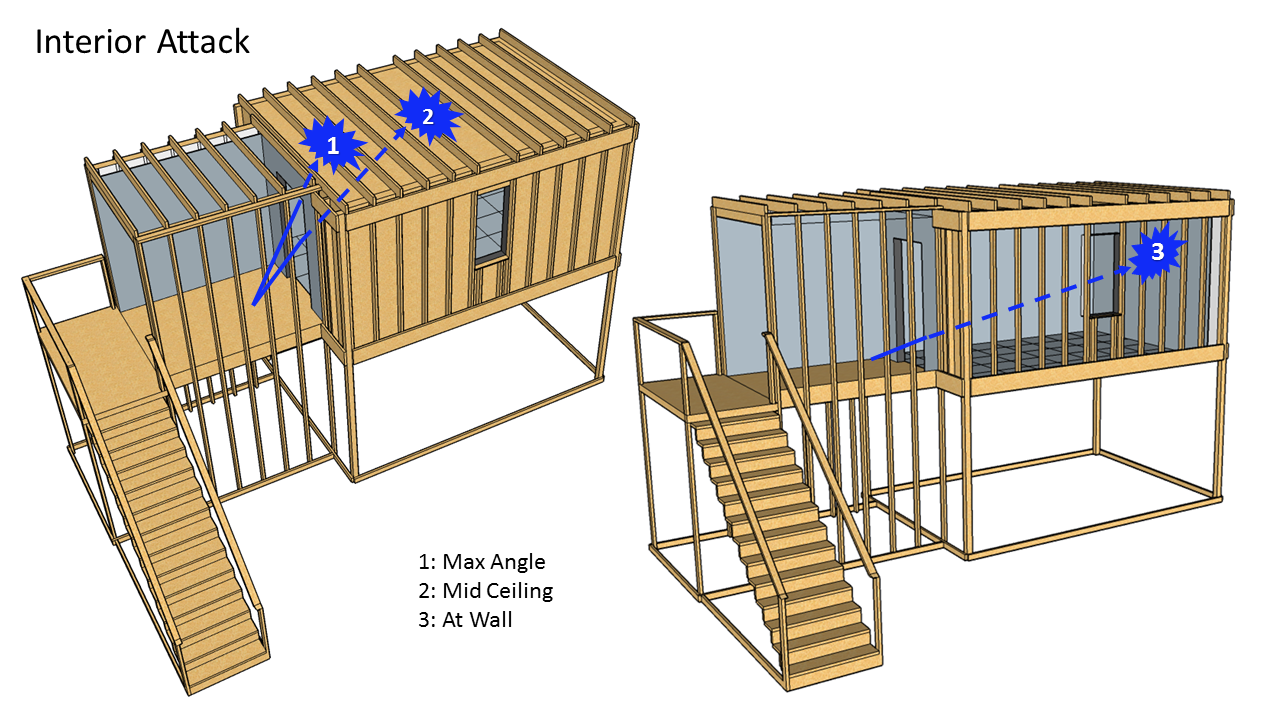
\includegraphics[width=\columnwidth]{Figures/Water_Distribution/Nozzle_Position_Int}
	\caption[Nozzle Direction, Interior Attack]{Nozzle Direction, Interior Attack.}
	\label{fig:Nozzle_Direction_Interior_Attack}
\end{figure}

\begin{table}[!ht]
\centering
\small
\caption{Interior Water Distribution Experiments}
\label{tab:Interior_Fire_Attack_Distribution_Experiments}
\begin{tabular}{ccccc}
\toprule[1.5pt]
Hose Stream Type & Nozzle Direction & Nozzle Movement & Nozzle Pressure (psi) & Flow Rate (gpm) \\ 
\midrule
Straight Stream   & Max Angle Ceiling   & O       & 100 & 150 \\
Straight Stream   & Max Angle Ceiling   & Fixed   & 100 & 150 \\
Straight Stream   & Mid Ceiling 		& Fixed   & 100 & 125 \\
Straight Stream   & Mid Ceiling 		& O       & 100 & 125 \\
Straight Stream   & Mid Ceiling 		& Z       & 100 & 125 \\
Straight Stream   & Mid Ceiling 		& T       & 100 & 125 \\
Straight Stream   & Mid Ceiling 		& Inverted U & 100 & 125 \\
Straight Stream   & Mid Ceiling 		& Fixed   & 100 & 150 \\
Straight Stream   & Mid Ceiling 		& O       & 100 & 150 \\
Straight Stream   & Mid Ceiling 		& Fixed   & 75 & 150 \\
Straight Stream   & Mid Ceiling 		& O & 75  & 150 \\
Straight Stream   & Mid Ceiling 		& Fixed   & 50 & 150 \\
Straight Stream   & Mid Ceiling 		& O & 50  & 150 \\
Straight Stream   & At Wall     		& Fixed   & 100 & 150 \\
Straight Stream   & At Wall     		& O       & 100 & 150 \\
Fog               & Mid Ceiling 		& Fixed   & 100 & 125 \\
Fog               & Mid Ceiling 		& Fixed   & 100 & 150 \\
Fog               & Mid Ceiling 		& O       & 100 & 150 \\
Fog               & Mid Ceiling 		& Fixed   & 75 & 150 \\
Fog               & Mid Ceiling 		& O & 75  & 150 \\
Fog               & Mid Ceiling 		& Fixed   & 50 & 150 \\
Fog               & Mid Ceiling 		& O & 50  & 150 \\
Fog               & Mid Ceiling 		& O       & 100 & 125 \\  
15/16 Smooth Bore & Max Angle Ceiling   & Fixed   & 50 & 180 \\
15/16 Smooth Bore & Max Angle Ceiling   & O & 50  & 180 \\
15/16 Smooth Bore & At Wall     		& Fixed   & 50 & 180 \\
15/16 Smooth Bore & At Wall     		& O & 50  & 180 \\
15/16 Smooth Bore & Mid Ceiling 		& Fixed   & 50 & 180 \\
15/16 Smooth Bore & Mid Ceiling 		& O & 50  & 180 \\
\bottomrule[1.25pt]
\end{tabular}
\end{table}

\clearpage

\subsection{Exterior Experiments}
\label{ext_tests}

The exterior experiments included two attack positions; one attack was from the fire floor and the second was from the floor below the fire. These are referred to as first floor and second floor attacks. The movable staircase to allowed for the variation between first floor and second floor suppression through the same window vent. The exterior experiments simulated a single room of fire in which an exterior attack was used. Similar to the interior testing, the hose stream type, the nozzle direction, and nozzle direction were varied for comparison. The differences in first floor and second floor attacks can been seen in Figures \ref{fig:Nozzle_Direction_Exterior_1st_Floor_Attack} and \ref{fig:Nozzle_Direction_Exterior_2nd_Floor_Attack}. 

There were five nozzle directions for the first floor exterior experiments: max angle ceiling, mid ceiling, min angle ceiling, max angle wall, and at wall. The max angle ceiling position was defined as the steepest angle the nozzle could be positioned at without the window soffit impacting the hose stream. The mid ceiling position was defined by the hose stream aimed at the center of the compartment in the 10~ft 5~in dimension. The min angle ceiling position was defined by the shallowest angle such the hose stream did not directly contact the wall. The max angle wall is similar to the max angle ceiling except it was defined as the steepest angle where the hose stream would impact the wall without the stream contacting the ceiling directly. The final position was aiming the stream at the position on the wall across from the window.

There were also five nozzle directions for the second floor exterior experiments: max angle ceiling, mid ceiling, min angle ceiling, max angle wall, and soffit. The first four positions were the same as the first floor exterior attack except that the starting position of the nozzle changed to be one story below the window vent. The fifth nozzle position, at soffit, was defined to be the maximum angle such that stream directed off the window soffit.

The exterior experiments are shown in Table~\ref{tab:Exterior_Fire_Attack_Distribution_Experiments}.

\begin{figure}[!ht]
	\centering
	\includegraphics[width=\columnwidth]{Figures/Water_Distribution/Nozzle_Position_ExtFirstfloor}
	\caption[Nozzle Direction, Exterior 1st Floor Attack]{Nozzle Direction, Exterior 1st Floor Attack.}
	\label{fig:Nozzle_Direction_Exterior_1st_Floor_Attack}
\end{figure}

\begin{figure}[!ht]
	\centering
	\includegraphics[width=\columnwidth]{Figures/Water_Distribution/Nozzle_Position_ExtSecondfloor}
	\caption[Nozzle Direction, Exterior 2nd Floor Attack]{Nozzle Direction, Exterior 2nd Floor Attack.}
	\label{fig:Nozzle_Direction_Exterior_2nd_Floor_Attack}
\end{figure}

\clearpage

\begin{table}[!ht]
\centering
\scriptsize
\caption{Exterior Water Distribution Experiments}
\label{tab:Exterior_Fire_Attack_Distribution_Experiments}
\begin{tabular}{lcccccl}
\toprule[1.5pt]
Floor & Hose Stream Type & Nozzle Direction & Nozzle Movement & Nozzle Pressure (psi) & Flow Rate (gpm) & Notes \\ 
\midrule

First  & Straight Stream  & Max Angle Ceiling      & Fixed              & 100 & 150 &   \\
First  & Straight Stream  & Max Angle Ceiling      & Fixed              & 100 & 150 &   \\
First  & Straight Stream  & Max Angle Ceiling      & Fixed              & 100 & 150 &   \\
First  & Straight Stream  & Max Angle Ceiling      & Fixed              & 100 & 150 &   \\
First  & Straight Stream  & Max Angle Ceiling      & Fixed              & 100 & 150 &   \\
First  & Straight Stream  & Max Angle Ceiling      & Fixed              & 100 & 150 &   \\
First  & Straight Stream  & Max Angle Ceiling      & Fixed              & 100 & 150 &   \\
First  & Straight Stream  & Max Angle Ceiling      & Fixed              & 100 & 150 & 1/2 Bail  \\
First  & Straight Stream  & Max Angle Ceiling      & Fixed              & 100 & 150 & 45~s Flow  \\
First  & Straight Stream  & Max Angle Ceiling      & Fixed              & 100 & 150 & 30~s Flow  \\
First  & Straight Stream  & Max Angle Ceiling      & Fixed              & 75  & 150 & 15~s Flow  \\
First  & Straight Stream  & Max Angle Ceiling      & Fixed              & 75  & 60 &   \\
First  & Straight Stream  & Max Angle Ceiling      & Fixed              & 50  & 185 &   \\
First  & Straight Stream  & Max Angle Ceiling      & Fixed              & 50  & 150 &   \\
First  & Straight Stream  & Max Angle Ceiling      & Fixed              & 25  & 150 &   \\
First  & Straight Stream  & Max Angle Ceiling      & Fixed              & 25  & 130 & 30~s Flow  \\
First  & Straight Stream  & Max Angle Ceiling      & Fixed              & 100 & 250 &   \\
First  & Straight Stream  & Max Angle Ceiling      & Sweeping           & 100 & 150 &   \\
First  & Straight Stream  & Max Angle Ceiling      & Wide Sweep         & 100 & 150 &   \\
First  & Straight Stream    & Mid Ceiling          & Fixed      		& 100 & 150 &   \\
First  & Straight Stream    & Min Angle Ceiling    & Fixed     		    & 100 & 150 &   \\
First  & Straight Stream    & Min Angle Ceiling    & Fixed      		& 100 & 250 &   \\
First  & Straight Stream    & Max Angle Wall       & Fixed     		    & 100 & 150 &   \\
First  & Straight Stream    & At Wall              & Fixed      		& 100 & 150 &   \\
First  & 15/16 Smooth Bore  & Max Angle Ceiling      & Fixed         	& 50 & 180 &   \\
First  & 15/16 Smooth Bore  & Max Angle Ceiling      & Sweeping      	& 50 & 180 &   \\
First  & 15/16 Smooth Bore  & Max Angle Ceiling      & Fixed        	& 50 & 180 & 1/2 Bail  \\
First  & 15/16 Smooth Bore  & Max Angle Ceiling      & Fixed        	& 30 & 150 &   \\
First  & 15/16 Smooth Bore  & Max Angle Ceiling      & Fixed        	& 15 & 130 &   \\
First  & 15/16 Smooth Bore  & Max Angle Ceiling      & Fixed        	& 10 & 100 &   \\
First  & 15/16 Smooth Bore  & Mid Ceiling            & Fixed 			& 50 & 180 &   \\
First  & 15/16 Smooth Bore  & Min Angle Ceiling      & Fixed			& 50 & 180 &   \\
First  & 15/16 Smooth Bore  & Max Angle Wall         & Fixed			& 50 & 180 &   \\
First  & 15/16 Smooth Bore  & At Wall                & Fixed 			& 50 & 180 &   \\
First  & 7/8 Smooth Bore    & Max Angle Ceiling      & Fixed         	& 50 & 150 &   \\
First  & 1 Smooth Bore      & Max Angle Ceiling      & Fixed        	& 50 & 210 &   \\
First  & 1 1/4 Smooth Bore  & Max Angle Ceiling      & Fixed         	& 50 & 260 &   \\
First  & Fog                & Max Angle Ceiling      & Fixed        	& 100 & 150 &   \\
First  & Straight Stream/Fog & Max Angle Ceiling    & Fixed/O           & 100 & 150 &   \\
\midrule
Second & Straight Stream    & Max Angle Ceiling      & Fixed                   & 100 & 150 &   \\
Second & Straight Stream    & Max Angle Ceiling      & Sweeping                & 100 & 150 &   \\
Second & Straight Stream    & Max Angle Ceiling      & Wide Sweep              & 100 & 150 &   \\
Second & Straight Stream    & Mid Ceiling            & Fixed                   & 100 & 150 &   \\
Second & Straight Stream    & Min Angle Ceiling      & Fixed                   & 100 & 150 &   \\
Second & Straight Stream    & Max Angle Wall         & Fixed                   & 100 & 150 &   \\
Second & Straight Stream    & Soffit         		 & Fixed                   & 100 & 150 &   \\
Second & 15/16 Smooth Bore  & Max Angle Ceiling      & Fixed                   & 50 & 180 &   \\
Second & 15/16 Smooth Bore  & Max Angle Ceiling      & Sweeping       	       & 50 & 180 &   \\
Second & 15/16 Smooth Bore  & Mid Ceiling            & Fixed                   & 50 & 180 &   \\
Second & 15/16 Smooth Bore  & Min Angle Ceiling      & Fixed                   & 50 & 180 &   \\
Second & 15/16 Smooth Bore  & Max Angle Wall         & Fixed                   & 50 & 180 &   \\
Second & 7/8 Smooth Bore    & Max Angle Ceiling      & Fixed                   & 50 & 150 &   \\
Second & 1 Smooth Bore      & Max Angle Ceiling      & Fixed                   & 50 & 210 &   \\
Second & Fog                & Max Angle Ceiling      & Fixed                   & 100 & 150 & 45~s Flow \\
Second & Fog                & Max Angle Ceiling      & Fixed/O                 & 100 & 150 &   \\
\bottomrule[1.25pt]
\end{tabular}
\end{table}

\chapter{Results}

The intent of the water flow experiments was to determine the location of the water within the compartment as a function of several common fire service nozzle configurations and application locations. Recall, the location of the water within the compartment was achieved using the ADD device (Section~\ref{sec:add_instrumentation}). To ensure that differences between distributions of water flux within the compartment could be quantified, it was important to confirm the repeatability of experiments. The first step was to compare the total volume of water measured in the ADD to the total volume of water expected. Table~\ref{Expected_vs._Experimental_Water_Differences} in Appendix~\ref{app:Water_Volume} shows the expected volume, experimentally measured volume, and percent difference. The average percent different for the experiments was 7.4~\%, within to the expected uncertainty described in Section~\ref{sec:add_instrumentation}. The second step was to compare repeatability between replicate tests.Four experiments utilizing a straight stream pattern from a combination nozzle flowing 150~gpm at 100~psi from a 1 3/4~in. hoseline from the exterior first floor position directed into the structure with a maximum angle were conducted to determine the variance in results. The average flux (gpm/ft$^2$) of water in each of the 48 collection bins for the four replicate experiments is shown in Figure~\ref{fig:Repeatability_Testing}. In each the ba{}r chart, bins with less than 0.05 gpm/ft$^2$ are grey, bins that are greater than 0.05~gpm/ft$^2$ but less than 3~gpm/ft$^2$ are colored blue, with more than 3~gpm/ft$^2$ but less than 6~gpm/ft$^2$ are colored green, with more than 6~gpm/ft$^2$ but less than 9~gpm/ft$^2$ are colored yellow, and bins with more than 9~gpm/ft$^2$ are colored red. The choice for the bottom threshold is to provide a relationship to residential sprinklers. According to NFPA 13D, a residential sprinkler system shall provide at least the flow required to produce a minimum discharge density of 0.05~gpm/ft$^2$~\cite{NFPA_13D}.

\begin{figure}[ht]
\begin{tabular*}{\textwidth}{lr}
\includegraphics[width=3.2in]{Script_Figures/ADD_Analysis/15-12-10_082039_Datafile_Rate_Straight_Stream_Exterior} &
\includegraphics[width=3.2in]{Script_Figures/ADD_Analysis/15-12-10_082423_Datafile_Rate_Straight_Stream_Exterior} \\
\includegraphics[width=3.2in]{Script_Figures/ADD_Analysis/15-12-10_083305_Datafile_Rate_Straight_Stream_Exterior} &
\includegraphics[width=3.2in]{Script_Figures/ADD_Analysis/15-12-10_083751_Datafile_Rate_Straight_Stream_Exterior} \\
\end{tabular*}
\caption[Water Flux for Straight Stream Exterior at Max Angle]{Water flux in each collection bin for a fixed exterior straight stream nozzle flowing 150~gpm at 100~psi from the first floor position directed into the structure with a maximum angle. The four bar charts are replicate tests of the same configuration.}
\label{fig:Repeatability_Testing}
\end{figure}

Qualitatively, the array of bars in each chart in Figure~\ref{fig:Repeatability_Testing} look similar to one another. However, to better compare the tests, a statistical approach known as an analysis of variance (ANOVA), was performed. Specifically, the Kruskal-Willis one-way ANOVA test was applied. The goal of this analysis was to quantify whether samples (in this case the flow rate of water in each bin) originate from the same distribution (are the configurations compared similar or different). The Kruskal-Willis analysis was selected because there is no prior assumption that the data is normally distributed. While this statistical analysis can compare $n$ number of data sets and identify if the data sets are statistically different, a limitation in all ANOVAs is the inability to identify which data sets are statistically different. The result of the ANOVA is a p-value. If the p-value is less than 0.05, the experiments being compared are statistically different. If the p-value is large, the experiments being compared are not statistically different.

For the straight stream experiments shown in Figure~\ref{fig:Repeatability_Testing}, a Kruskal-Willis ANOVA test was applied based on average flow rate of water into each collection bin. The resulting p-value was 0.902 average water flux. The high p-value means that the 4 straight stream flow patterns cannot be distinguished from one another. In other words, these experiments can be considered as repeatable.

Confirmation of repeatability, allowed for the exploration of additional comparisons within the data. The three main comparison sets were variation of hose stream type, variation of nozzle direction, and variation of the flow pressure/flow rate. 

\section{Comparison of Impact of Hose Stream Type}

The hose stream type experiments were designed to quantify the distributions of water flux from a straight stream, smooth bore stream, and a narrow fog stream. Six configuration sets were analyzed. Within each configuration set, the nozzle direction, nozzle movement, and nozzle pressure/flow rate were fixed. Table~\ref{tab:add_hosestream} shows the results from the ANOVA test based on a comparison of the distribution of the average water flux (gpm/ft$^2$) within the compartment. The configuration column in the table provides the location (and floor) of the nozzle, the nozzle position, and the nozzle movement. Note that for the exterior water flow experiments with a sweep pattern, only a straight stream and smooth bore hose stream are compared. The pattern from a fog stream could typically encompass the entire window opening, depending on the size of the opening and the distance from the opening. In these experiments, the fog stream enclosed the window, therefore only a fixed pattern was studied. 

\begin{table}[!ht]
\centering
\small
\caption{Variation of Hose Stream Types: Straight Stream, Smooth Bore Stream, Fog Stream}
\label{tab:add_hosestream}
\begin{tabular}{lccc}
\toprule[1.5pt]
Configuration & \# of Tests & P Value Rate & Different \\ 
\midrule
 Interior, Mid Ceiling, Fixed Pattern                  & 3          & 2.8E-06 & \checkmark \\
 Interior, Mid Ceiling, `O' Pattern                    & 3          & 1.0E-04 & \checkmark \\
 1st Floor Exterior, Max Angle Ceiling, Fixed Pattern  & 3          & 0.051   &            \\
 2nd Floor Exterior, Max Angle Ceiling, Fixed Pattern  & 3          & 0.048   & \checkmark \\
 1st Floor Exterior, Max Angle Ceiling, Sweep Pattern  & 2          & 0.275   &            \\
 2nd Floor Exterior, Max Angle Ceiling, Sweep Pattern  & 2          & 0.501   &            \\
\bottomrule[1.25pt]
\end{tabular}
\end{table}

The results of the statistical analysis identified that 3 of the 6 hose stream comparisons showed statistical difference between the distributions of average water flux. Here, statistical difference means that the resulting distributions likely originated from different sources. In other words, the hose streams that produced the water flux distributions are not the same. For the interior tests, both the fixed pattern and `O' pattern showed statistical differences (Figures~\ref{fig:Interior_Varying_Nozzle_Types_Fixed_Pattern} and \ref{fig:Interior_Varying_Nozzle_Types_O_Pattern}). 

The distributions in Figure~~\ref{fig:Interior_Varying_Nozzle_Types_Fixed_Pattern} are similar in the the majority of the water flowed into the buckets opposite the doorway and these buckets all had rates greater than a typical residential sprinkler. For the straight stream and smooth bore stream the profile of water flux along the wall in fairly flat. In the case of the fog stream, the flux profile is parabolic with a peak flow at the center and minimums at the corners of the room. For the smooth bore stream, note that along the walls parallel to the flow, there are several buckets that exceed 0.05~gpm/ft$^2$, which the other two hose stream types do not produce. 

Comparison of interior experiments with the `O' pattern also yielded a p-test value that indicates the streams are different. While the water flux data in Figure~\ref{fig:Interior_Varying_Nozzle_Types_O_Pattern}, shows increased water coverage within the compartment compared to a fixed stream, there are differences within the hose stream types. The straight stream and fog stream have more pronounced water flux at the corners of the room while the smooth bore steam has a flatter profile. The `O' pattern smooth bore stream has more floor coverage in excess of 0.05~gpm/ft$^2$ especially along the walls parallel to the stream direction.


\begin{figure}[!ht]
\begin{tabular*}{\textwidth}{lr}
\includegraphics[width=3.2in]{Script_Figures/ADD_Analysis/15-12-09_121955_Datafile_Rate_Straight_Stream_Interior} &
\includegraphics[width=3.2in]{Script_Figures/ADD_Analysis/15-12-09_144839_Datafile_Rate_15_16in_Smooth_Bore_Interior} \\
\end{tabular*}
\centering
\includegraphics[width=3.2in]{Script_Figures/ADD_Analysis/15-12-09_123142_Datafile_Rate_Fog_Interior} \\
\caption[Water Flux for Varying Interior Fixed Pattern Hose Stream Types]{Water flux in each collection bin for interior fixed pattern flow at the mid-ceiling direction for a straight stream (upper left), smooth bore stream (upper right), and fog stream (bottom middle).}
\label{fig:Interior_Varying_Nozzle_Types_Fixed_Pattern}
\end{figure}

\begin{figure}[ht]
\begin{tabular*}{\textwidth}{lr}
\includegraphics[width=3.2in]{Script_Figures/ADD_Analysis/15-12-09_122551_Datafile_Rate_Straight_Stream_Interior} &
\includegraphics[width=3.2in]{Script_Figures/ADD_Analysis/15-12-09_145534_Datafile_Rate_15_16in_Smooth_Bore_Interior} \\
\end{tabular*}
\centering
\includegraphics[width=3.2in]{Script_Figures/ADD_Analysis/15-12-09_123636_Datafile_Rate_Fog_Interior}
\caption[Water Flux for Varying Interior `O' Pattern Hose Stream Types]{Water volume in each collection bin for interior `O' pattern flow at the mid-ceiling direction for a straight stream (upper left), smooth bore stream (upper right), and fog stream (bottom middle).}
\label{fig:Interior_Varying_Nozzle_Types_O_Pattern}
\end{figure}

\clearpage

Statistical tests of fixed pattern exterior experiments for first and second floor locations comparing hose stream types, resulted in one set that showed statistical similarly and one set that showed statistical difference. The p-test value of 0.051 indicated that the flux data are similar and Figure~\ref{fig:Exterior_FirstFloor_Fixed_Varying_Nozzle} shows the flux data for the straight stream, smooth bore stream and fog stream. While the smooth bore stream showed increased water flow around the perimeter, all three hose streams show similar overall patterns. 

The second floor exterior experiments examining straight stream, smooth bore stream, and fog stream resulted in a p-value that indicated the hose stream types produced different water flux distributions. Figure~\ref{fig:Exterior_SecondFloor_Fixed_Varying_Nozzle} shows the flux distributions for the three hose stream types. The straight stream and smooth bore stream show similar flows with a flat profile along the wall opposite the window and values all above the 0.05~gpm/ft$^2$ residential sprinkler threshold, the fog stream produced a noticeably different pattern. The fog stream shows a parabolic pattern along the wall opposite the window and significantly less water flow around the perimeter of the compartment. 

\begin{figure}[ht]
\begin{tabular*}{\textwidth}{lr}
\includegraphics[width=3.2in]{Script_Figures/ADD_Analysis/15-12-08_113237_Datafile_Rate_Straight_Stream_Exterior} &
\includegraphics[width=3.2in]{Script_Figures/ADD_Analysis/15-12-08_101028_Datafile_Rate_15_16in_Smooth_Bore_Exterior} \\
\end{tabular*}
\centering
\includegraphics[width=3.2in]{Script_Figures/ADD_Analysis/15-12-08_121806_Datafile_Rate_Fog_Exterior}
\caption[Water Flux for Varying Exterior First Floor Fixed Pattern Hose Stream Types]{Water flux in each collection bin for exterior first floor fixed pattern flow at the max angle direction for a straight stream (upper left), smooth bore stream (upper right), and fog stream (bottom middle).}
\label{fig:Exterior_FirstFloor_Fixed_Varying_Nozzle}
\end{figure}

\begin{figure}[ht]
\begin{tabular*}{\textwidth}{lr}
\includegraphics[width=3.2in]{Script_Figures/ADD_Analysis/15-12-07_145156_Datafile_Rate_Straight_Stream_Exterior} &
\includegraphics[width=3.2in]{Script_Figures/ADD_Analysis/15-12-07_111118_Datafile_Rate_15_16in_Smooth_Bore_Exterior} \\
\end{tabular*}
\centering
\includegraphics[width=3.2in]{Script_Figures/ADD_Analysis/15-12-07_155751_Datafile_Rate_Fog_Exterior}
\caption[Water Flux for Varying Exterior Second Floor Fixed Pattern Hose Stream Types]{Water volume in each collection bin for exterior second floor fixed pattern flow at the max angle direction for a straight stream (upper left), smooth bore stream (upper right), and fog stream (bottom middle).}
\label{fig:Exterior_SecondFloor_Fixed_Varying_Nozzle}
\end{figure}

\clearpage

The final two comparison sets were both exterior streams (one first floor set and one second floor set) at the max angle on the ceiling with sweeping patterns. Again, only the straight stream and smooth bore streams were compared for cases where the nozzle pattern was a sweeping motion from an exterior position. In both cases, the first floor and second floor location, the analysis revealed that the straight stream and smooth bore stream produce statistically similar distributions. Figures~\ref{fig:Exterior_FirstFloor_O_Varying_Nozzle} and \ref{fig:Exterior_SecondFloor_O_Varying_Nozzle} confirm the similarity in the water flux distributions.

\begin{figure}[ht]
\begin{tabular*}{\textwidth}{lr}
\includegraphics[width=3.2in]{Script_Figures/ADD_Analysis/15-12-08_113716_Datafile_Rate_Straight_Stream_Exterior} &
\includegraphics[width=3.2in]{Script_Figures/ADD_Analysis/15-12-08_101825_Datafile_Rate_15_16in_Smooth_Bore_Exterior}
\end{tabular*}
\caption[Water Flux for Varying Exterior First Floor Sweeping Pattern Hose Stream Types]{Water flux in each collection bin for exterior first floor sweeping pattern flow at the max angle direction for a straight stream (left) and smooth bore stream (right).}
\label{fig:Exterior_FirstFloor_O_Varying_Nozzle}
\end{figure}

\begin{figure}[ht]
\begin{tabular*}{\textwidth}{lr}
\includegraphics[width=3.2in]{Script_Figures/ADD_Analysis/15-12-07_145842_Datafile_Rate_Straight_Stream_Exterior} &
\includegraphics[width=3.2in]{Script_Figures/ADD_Analysis/15-12-07_121014_Datafile_Rate_15_16in_Smooth_Bore_Exterior}
\end{tabular*}
\caption[Water Flux for Varying Exterior Second Floor Sweeping Pattern Hose Stream Types]{Water volume in each collection bin for exterior second floor sweeping pattern flow at the max angle direction for a straight stream (left) and smooth bore stream (right).}
\label{fig:Exterior_SecondFloor_O_Varying_Nozzle}
\end{figure}


\section{Comparison of Impact of Nozzle Direction}

The second comparison was to quantify the impact of nozzle direction on water distribution within the compartment. Referring back to Figures~\ref{fig:Nozzle_Direction_Interior_Attack}, \ref{fig:Nozzle_Direction_Exterior_1st_Floor_Attack}, and \ref{fig:Nozzle_Direction_Exterior_2nd_Floor_Attack} there are 3, 5, and 5 nozzle directions for the interior experiments, the exterior first floor experiments, and the exterior second floor experiments, respectively. Table~\ref{tab:add_nozzleposition} shows the p-test values comparing average water flux per collection bin  for the nozzle direction comparison experiments. For the case where the nozzle direction was the same, but the starting floor was varied (Configuration: 1st and 2nd Floor, Exterior, Straight Stream) the resulting distributions were similar. In all comparisons where the nozzle location was fixed and the nozzle direction was varied, there was enough variation in the water flux data to indicate that the data was statistically different. 

\begin{table}[!ht]
\centering
\small
\caption{Variation of Nozzle Directions}
\label{tab:add_nozzleposition}
\begin{tabular}{lccc}
\toprule[1.5pt]
Configuration & \# of Tests & P Value Rate & Different \\ 
\midrule
 Interior, Smooth Bore, Fixed Pattern                  & 3          & 1.4E-04 & \checkmark  \\
 Interior, Straight Stream, Fixed Pattern              & 3          & 2.9E-08 & \checkmark  \\
 Interior, Smooth Bore, `O' Pattern                    & 3          & 2.3E-04 & \checkmark  \\
 Interior, Straight Stream, `O' Pattern                & 3          & 5.8E-04 & \checkmark  \\
 1st Floor Exterior, Straight Stream, Fixed Pattern    & 5          & 1.1E-07 & \checkmark  \\
 1st Floor Exterior, Smooth Bore Fixed Pattern         & 5          & 6.2E-07 & \checkmark  \\
 2nd Floor Exterior, Straight Stream Fixed Pattern     & 5          & 2.9E-09 & \checkmark  \\
 2nd Floor Exterior, Smooth Bore Fixed Pattern         & 4          & 1.2E-05 & \checkmark  \\
 1st and 2nd Floor, Exterior, Straight Stream          & 2          & 0.133   &             \\
\bottomrule[1.25pt]
\end{tabular}
\end{table}

For the interior tests, there were three nozzle directions examined: max angle ceiling, mid ceiling, and at wall (Figure~\ref{fig:Nozzle_Direction_Interior_Attack}). The fixed pattern interior smooth bore stream and straight stream tests both show variation in the data (Table~\ref{tab:add_nozzleposition}) which is also visualized in the water flux charts, Figures~\ref{fig:Interior_Varying_Nozzle_Direction_SB_Fixed_Pattern} and \ref{fig:Interior_Varying_Nozzle_Direction_SS_Fixed_Pattern} respectively. Specifically, the max angle ceiling direction for both hose stream types resulted in the perimeter of the compartment exceeding the 0.05~gpm/ft$^2$ water flux of residential sprinklers. At the mid ceiling and wall positions, the water flow is more localized along the wall opposite the doorway.

The interior `O' pattern smooth bore stream and straight stream experiments were similar to the fixed pattern, Figures~\ref{fig:Interior_Varying_Nozzle_Direction_SB_O_Pattern} and \ref{fig:Interior_Varying_Nozzle_Direction_SS_O_Pattern}, respectively. For both hose stream types, moving the nozzle through the three directions resulted in statistically different water flux distributions. Again, the mid ceiling and wall direction showed water concentrated along the wall opposite the doorway while the max angle showed water distributed around the perimeter. 

\begin{figure}[ht]
\begin{tabular*}{\textwidth}{lr}
\includegraphics[width=3.2in]{Script_Figures/ADD_Analysis/15-12-09_145932_Datafile_Rate_15_16in_Smooth_Bore_Interior} &
\includegraphics[width=3.2in]{Script_Figures/ADD_Analysis/15-12-09_144839_Datafile_Rate_15_16in_Smooth_Bore_Interior} \\
\end{tabular*}
\centering
\includegraphics[width=3.2in]{Script_Figures/ADD_Analysis/15-12-09_142948_Datafile_Rate_15_16in_Smooth_Bore_Interior}
\caption[Water Flux for Varying Nozzle Direction with Fixed Interior Smooth Bore Stream]{Water flux in each collection bin for an interior smooth bore stream with a fixed pattern at three nozzle directions: max angle ceiling (top left), mid ceiling (top right) and at wall (bottom).}
\label{fig:Interior_Varying_Nozzle_Direction_SB_Fixed_Pattern}
\end{figure}

\begin{figure}[ht]
\begin{tabular*}{\textwidth}{lr}
\includegraphics[width=3.2in]{Script_Figures/ADD_Analysis/15-12-09_152435_Datafile_Rate_Straight_Stream_Interior} &
\includegraphics[width=3.2in]{Script_Figures/ADD_Analysis/15-12-09_112850_Datafile_Rate_Straight_Stream_Interior} \\
\end{tabular*}
\centering
\includegraphics[width=3.2in]{Script_Figures/ADD_Analysis/15-12-09_151401_Datafile_Rate_Straight_Stream_Interior} 
\caption[Water Flux for Varying Nozzle Direction with Fixed Interior Straight Stream]{Water flux in each collection bin for an interior straight stream with a fixed pattern at three nozzle directions: max angle ceiling (top left), mid ceiling (top right) and at wall (bottom).}
\label{fig:Interior_Varying_Nozzle_Direction_SS_Fixed_Pattern}
\end{figure}

\begin{figure}[ht]
\begin{tabular*}{\textwidth}{lr}
\includegraphics[width=3.2in]{Script_Figures/ADD_Analysis/15-12-09_150300_Datafile_Rate_15_16in_Smooth_Bore_Interior} &
\includegraphics[width=3.2in]{Script_Figures/ADD_Analysis/15-12-09_145534_Datafile_Rate_15_16in_Smooth_Bore_Interior} \\
\end{tabular*}
\centering
\includegraphics[width=3.2in]{Script_Figures/ADD_Analysis/15-12-09_144524_Datafile_Rate_15_16in_Smooth_Bore_Interior}
\caption[Water Flux for Varying Nozzle Direction with `O' Pattern Interior Smooth Bore Stream]{Water flux in each collection bin for an interior smooth bore stream with an `O' pattern at three nozzle directions: max angle ceiling (top left), mid ceiling (top right) and at wall (bottom).}
\label{fig:Interior_Varying_Nozzle_Direction_SB_O_Pattern}
\end{figure}

\begin{figure}[ht]
\begin{tabular*}{\textwidth}{lr}
\includegraphics[width=3.2in]{Script_Figures/ADD_Analysis/15-12-09_153038_Datafile_Rate_Straight_Stream_Interior} &
\includegraphics[width=3.2in]{Script_Figures/ADD_Analysis/15-12-09_113335_Datafile_Rate_Straight_Stream_Interior} \\
\end{tabular*}
\centering
\includegraphics[width=3.2in]{Script_Figures/ADD_Analysis/15-12-09_151823_Datafile_Rate_Straight_Stream_Interior}
\caption[Water Flux for Varying Nozzle Direction with `O' Interior Straight Stream]{Water volume in each collection bin for an interior straight stream with an 'O' pattern at three nozzle directions: max angle ceiling (top left), mid ceiling (top right) and at wall (bottom).}
\label{fig:Interior_Varying_Nozzle_Direction_SS_O_Pattern}
\end{figure}

\clearpage

The first floor exterior experiments used 5 different nozzle directions: max angle ceiling, mid ceiling, min angle ceiling, max angle wall, and at wall. Statistical analysis indicated that the water flux distributions produced from the 5 nozzle direction are not the same for both the smooth bore stream and straight stream experiments. Figure~\ref{fig:Exterior_First_Floor_Varying_Nozzle_Directions_SB_Fixed_Pattern} shows the water flux distribution for the 5 directions for the smooth bore stream while Figure~\ref{fig:Exterior_First_Floor_Varying_Nozzle_Directions_SS_Fixed_Pattern} shows the water volume distributions for the straight stream. For both hose stream types, the mid ceiling and min angle ceiling directions indicate that the majority of the water accumulated in the bins along the wall opposite the window. When the direction became steeper (max angle ceiling) the water was distributed around the perimeter, similar to the interior experiments. When the direction was at the two wall positions a broader distribution occurred. Comparable to the other directions there was still significant flow along the wall opposite the nozzle, but the two ceiling positions showed a broader distribution of water flow, specifically towards window where the nozzle was positioned.

The smooth bore and straight stream second floor exterior experiments were similar to the first floor exterior experiments. Changes in nozzle position produced water flux data that was statistically different. Figure~\ref{fig:Exterior_Second_Floor_Varying_Nozzle_Directions_SB_Fixed_Pattern} shows the results of the water flux distributions for 4 smooth bore directions and \ref{fig:Exterior_Second_Floor_Varying_Nozzle_Directions_SS_Fixed_Pattern} shows the results of the water flux distributions for 5 straight stream directions. The smooth bore stream max angle ceiling and max angle wall showed the largest spread of water flux, however with different patterns. The max angle ceiling showed a perimeter biased distribution (much like the interior and fire floor exterior max angle distributions) while the max angle wall had flux greater than 0.05~gpm/ft$^2$ over two thirds the rows of the collection buckets with the majority of the flow in the two rows along the wall opposite the window. The mid ceiling and mid angle ceiling both showed concentrated water flows along the wall opposite the window

Second floor straight stream experiments had similar distributions to the smooth bore stream except that a fifth nozzle direction was included. The exterior straight stream second floor soffit experiment showed the flattest, most disperse distribution of the the nozzle directions tested.

\begin{figure}[ht]
\begin{tabular*}{\textwidth}{lr}
\includegraphics[width=3.2in]{Script_Figures/ADD_Analysis/15-12-08_101028_Datafile_Rate_15_16in_Smooth_Bore_Exterior} &
\includegraphics[width=3.2in]{Script_Figures/ADD_Analysis/15-12-08_102802_Datafile_Rate_15_16in_Smooth_Bore_Exterior} \\
\includegraphics[width=3.2in]{Script_Figures/ADD_Analysis/15-12-08_103414_Datafile_Rate_15_16in_Smooth_Bore_Exterior} &
\includegraphics[width=3.2in]{Script_Figures/ADD_Analysis/15-12-08_104150_Datafile_Rate_15_16in_Smooth_Bore_Exterior} \\
\end{tabular*}
\centering
\includegraphics[width=3.2in]{Script_Figures/ADD_Analysis/15-12-08_104620_Datafile_Rate_15_16in_Smooth_Bore_Exterior} \\
\caption[Water Flux for Varying Nozzle Direction with Fixed First Floor Exterior Smooth Bore Stream]{Water flux in each collection bin for a first floor exterior smooth bore stream with a fixed pattern at five nozzle directions: max angle ceiling (top left), mid ceiling (top right), min angle ceiling (middle left), min angle at wall (middle right), and at wall (bottom).}
\label{fig:Exterior_First_Floor_Varying_Nozzle_Directions_SB_Fixed_Pattern}
\end{figure}

\begin{figure}[ht]
\begin{tabular*}{\textwidth}{lr}
\includegraphics[width=3.2in]{Script_Figures/ADD_Analysis/15-12-08_113237_Datafile_Rate_Straight_Stream_Exterior} &
\includegraphics[width=3.2in]{Script_Figures/ADD_Analysis/15-12-08_114905_Datafile_Rate_Straight_Stream_Exterior} \\
\includegraphics[width=3.2in]{Script_Figures/ADD_Analysis/15-12-08_120311_Datafile_Rate_Straight_Stream_Exterior} &
\includegraphics[width=3.2in]{Script_Figures/ADD_Analysis/15-12-08_121011_Datafile_Rate_Straight_Stream_Exterior} \\
\end{tabular*}
\centering
\includegraphics[width=3.2in]{Script_Figures/ADD_Analysis/15-12-08_121425_Datafile_Rate_Straight_Stream_Exterior} \\
\caption[Water Flux for Varying Nozzle Direction with Fixed First Floor Exterior Straight Stream]{Water flux in each collection bin for a first floor exterior straight stream with a fixed pattern at five nozzle directions: max angle ceiling (top left), mid ceiling (top right), min angle ceiling (middle left), min angle at wall (middle right), and at wall (bottom).}
\label{fig:Exterior_First_Floor_Varying_Nozzle_Directions_SS_Fixed_Pattern}
\end{figure}

\begin{figure}[ht]
\begin{tabular*}{\textwidth}{lr}
\includegraphics[width=3.2in]{Script_Figures/ADD_Analysis/15-12-07_111118_Datafile_Rate_15_16in_Smooth_Bore_Exterior} &
\includegraphics[width=3.2in]{Script_Figures/ADD_Analysis/15-12-07_122135_Datafile_Rate_15_16in_Smooth_Bore_Exterior} \\
\includegraphics[width=3.2in]{Script_Figures/ADD_Analysis/15-12-07_140034_Datafile_Rate_15_16in_Smooth_Bore_Exterior} &
\includegraphics[width=3.2in]{Script_Figures/ADD_Analysis/15-12-07_141333_Datafile_Rate_15_16in_Smooth_Bore_Exterior} \\
\end{tabular*}
\caption[Water Flux for Varying Nozzle Direction with Fixed Second Floor Exterior Smooth Bore Stream]{Water flux in each collection bin for a second floor exterior smooth bore stream with a fixed pattern at four nozzle directions: max angle ceiling (top left), mid ceiling (top right), min angle ceiling (bottom left), and max angle wall (bottom left)}
\label{fig:Exterior_Second_Floor_Varying_Nozzle_Directions_SB_Fixed_Pattern}
\end{figure}

\begin{figure}[ht]
\begin{tabular*}{\textwidth}{lr}
\includegraphics[width=3.2in]{Script_Figures/ADD_Analysis/15-12-07_145156_Datafile_Rate_Straight_Stream_Exterior} &
\includegraphics[width=3.2in]{Script_Figures/ADD_Analysis/15-12-07_151630_Datafile_Rate_Straight_Stream_Exterior} \\
\includegraphics[width=3.2in]{Script_Figures/ADD_Analysis/15-12-07_152028_Datafile_Rate_Straight_Stream_Exterior} &
\includegraphics[width=3.2in]{Script_Figures/ADD_Analysis/15-12-07_155226_Datafile_Rate_Straight_Stream_Exterior} \\
\end{tabular*}
\centering
\includegraphics[width=3.2in]{Script_Figures/ADD_Analysis/15-12-07_151001_Datafile_Rate_Straight_Stream_Exterior}
\caption[Water Flux for Varying Nozzle Direction with Fixed Second Floor Exterior Straight Stream]{Water flux in each collection bin for a second floor exterior straight stream with a fixed pattern at five nozzle directions: max angle ceiling (top left), mid ceiling (top right), min angle ceiling (middle left), max angle wall (middle right), and soffit (bottom).}
\label{fig:Exterior_Second_Floor_Varying_Nozzle_Directions_SS_Fixed_Pattern}
\end{figure}

\clearpage
Exterior, max angle ceiling straight streams, one from the first floor position and one from the second floor position, were compared. In this case, the stochastic test showed that the water distributions cannot be considered to be different. Figure~\ref{fig:Exterior_First_Floor_Second_Floor} shows the water flux distribution both cases.

\begin{figure}[ht]
\includegraphics[width=3.2in]{Script_Figures/ADD_Analysis/15-12-08_113237_Datafile_Rate_Straight_Stream_Exterior}
\includegraphics[width=3.2in]{Script_Figures/ADD_Analysis/15-12-07_145156_Datafile_Rate_Straight_Stream_Exterior} \\ 
\caption[Water Flux for Same Nozzle Direction Varying Exterior Floor]{Water flux in each collection bin for a first floor exterior straight stream at max angle ceiling (left) and a second floor exterior straight stream at max angle ceiling(right).}
\label{fig:Exterior_First_Floor_Second_Floor}
\end{figure}

\section{Comparison of Impact of Pressure and  Flow Rate}

The third set of analysis was to quantify the impact of nozzle pressure and nozzle flow rate on water distribution within the compartment. Table~\ref{tab:add_pressure} shows the statistical comparison results for water flux distributions. 

\begin{table}[!ht]
\centering
\footnotesize
\caption{Variation of Nozzle Pressure/Flowrate}
\label{tab:add_pressure}
\begin{tabular}{lccc}
\toprule[1.5pt]
Configuration & \# of Tests & P Value Rate & Different \\ 
\midrule
 Interior, Straight Stream, Mid Ceiling                      & 3   & 0.190   &            \\
 Interior, Fog Stream, Mid Ceiling                           & 3   & 0.196   &            \\
 1st Floor Exterior, Smooth Bore, Max Angle Ceiling          & 3   & 0.815   &            \\
 1st Floor Exterior Smooth Bore, Vary Tip Size               & 3   & 0.255   &            \\
 1st Floor Exterior, Straight Stream, Varying Pressure Disc  & 3   & 0.211   &            \\
 1st Floor Exterior, Varying Stream, Varying Hose Diameter   & 2   & 0.523   &            \\
 1st Floor Exterior, Smooth Bore, Varying Bail               & 2   & 5.8E-4  & \checkmark \\
\bottomrule[1.25pt]
\end{tabular}
\end{table}

Three comparisons examined the impact of changing water pressure: on a straight stream (Fig.~\ref{fig:Interior_Varying_Nozzle_Pressure_SS_Fixed_Pattern}), on a fog stream (Fig.~\ref{fig:Interior_Varying_Nozzle_Pressure_Fog_Fixed_Pattern}) and on a smooth bore stream (Fig.~\ref{fig:Exterior_First_Floor_Varying_Nozzle_Pressure_SB_Fixed_Pattern}). For each of these three hose stream types, the statistical analysis of the results of flow rate revealed that varying pressure did not result in distinctly different water flux distributions. The straight stream experiments were conducted at 100~psi, 75~psi, and 50~psi. For all three pressures, the water flux is similar in position (along the wall opposite the door) and profile (cf. Figure~\ref{fig:Interior_Varying_Nozzle_Pressure_SS_Fixed_Pattern}). The fog nozzle experiments were conducted at the same three pressures as the straight stream: 100~psi, 75~psi, and 50~psi. The distributions, shown in Figure~\ref{fig:Interior_Varying_Nozzle_Pressure_Fog_Fixed_Pattern}, all have similar parabolic profiles along the wall opposite the doorway. For the smooth bore stream, three flow rates were compared: 180~gpm at 50~psi, 150~gpm at 30~psi, and 130~gpm at 15~psi. In these cases, the total water flowed was decreased with decreased flow rate, but as Figure~\ref{fig:Exterior_First_Floor_Varying_Nozzle_Pressure_SB_Fixed_Pattern} shows, the distributions are similar. 

\begin{figure}[ht]
\begin{tabular*}{\textwidth}{lr}
\includegraphics[width=3.2in]{Script_Figures/ADD_Analysis/15-12-09_112850_Datafile_Rate_Straight_Stream_Interior} &
\includegraphics[width=3.2in]{Script_Figures/ADD_Analysis/15-12-09_115707_Datafile_Rate_Straight_Stream_Interior} \\
\end{tabular*}
\centering
\includegraphics[width=3.2in]{Script_Figures/ADD_Analysis/15-12-09_121955_Datafile_Rate_Straight_Stream_Interior}
\caption[Water Flux Varying Pressure with Straight Stream]{Water flux in each collection bin for an interior straight stream with a fixed pattern at 150~gpm with 100~psi (top left), 75~psi (top right) and 50~psi (bottom).}
\label{fig:Interior_Varying_Nozzle_Pressure_SS_Fixed_Pattern}
\end{figure}

\begin{figure}[ht]
\begin{tabular*}{\textwidth}{lr}
\includegraphics[width=3.2in]{Script_Figures/ADD_Analysis/15-12-09_113802_Datafile_Rate_Fog_Interior} &
\includegraphics[width=3.2in]{Script_Figures/ADD_Analysis/15-12-09_120821_Datafile_Rate_Fog_Interior} \\
\end{tabular*}
\centering
\includegraphics[width=3.2in]{Script_Figures/ADD_Analysis/15-12-09_123142_Datafile_Rate_Fog_Interior}
\caption[Water Flux Varying Pressure with Fog Stream]{Water flux in each collection bin for an interior fog stream with a fixed pattern at 150~gpm with 100~psi (top left), 75~psi (top right) and 50~psi (bottom).}
\label{fig:Interior_Varying_Nozzle_Pressure_Fog_Fixed_Pattern}
\end{figure}

\begin{figure}[ht]
\begin{tabular*}{\textwidth}{lr}
\includegraphics[width=3.2in]{Script_Figures/ADD_Analysis/15-12-08_101028_Datafile_Rate_15_16in_Smooth_Bore_Exterior} &
\includegraphics[width=3.2in]{Script_Figures/ADD_Analysis/15-12-08_154306_Datafile_Rate_15_16in_Smooth_Bore_Exterior} \\
\end{tabular*}
\centering
\includegraphics[width=3.2in]{Script_Figures/ADD_Analysis/15-12-08_154812_Datafile_Rate_15_16in_Smooth_Bore_Exterior}
\caption[Water Flux Varying Pressure with Smooth Bore Stream]{Water flux in each collection bin for a first floor exterior smooth bore a fixed pattern with 180~gpm at 50~psi (top left), 150~gpm at 30~psi (top right) and 130~gpm at 15~psi (bottom).}
\label{fig:Exterior_First_Floor_Varying_Nozzle_Pressure_SB_Fixed_Pattern}
\end{figure}

\clearpage

In addition to examining a fixed smooth bore nozzle with varying pressure, three smooth bore nozzles with different sizes were examined. The three configurations were a 1~in. tip that flowed 210~gpm at 50~psi, 15/16~in. tip that flowed 180~gpm at 50~psi, and a 7/8~in. tip that flow 150~gpm at 50~psi. Variation of tip size resulted in water flux distributions that could not be distinguished from one another. Figure~\ref{fig:Exterior_Second_Floor_Varying_Flow_Rates_SB_Fixed_Pattern} shows the water flux results for the three experiments.

\begin{figure}[ht]
\begin{tabular*}{\textwidth}{lr}
\includegraphics[width=3.2in]{Script_Figures/ADD_Analysis/15-12-07_143828_Datafile_Rate_1in_Smooth_Bore_Exterior} &
\includegraphics[width=3.2in]{Script_Figures/ADD_Analysis/15-12-07_111118_Datafile_Rate_15_16in_Smooth_Bore_Exterior} \\
\end{tabular*}
\centering
\includegraphics[width=3.2in]{Script_Figures/ADD_Analysis/15-12-07_143141_Datafile_Rate__7_8in_Smooth_Bore_Exterior}
\caption[Water Flux Varying Tip Size for Smooth Bore Nozzle]{Water flux in each collection bin for an exterior smooth bore stream with a fixed pattern with a 1~in. tip (top left), 15/16~in. tip (top right) and 7/8~in. tip (bottom).}
\label{fig:Exterior_Second_Floor_Varying_Flow_Rates_SB_Fixed_Pattern}
\end{figure}

To compare the impact of changing pressure disc options in a combination nozzle, three first floor exterior straight stream experiments at the max angle nozzle direction were compared. The three settings were 150~gpm at 100~psi, 185~gpm at 50~psi, and 150~gpm at 50~psi. Figure~\ref{fig:Exterior_First_Floor_Varying_Nozzle_Pressure_SS_Fixed_Pattern} shows the water flux patterns that are similar to one another, which is confirmed by the statistical analysis indicating the distributions are similar.   

\begin{figure}[ht]
\begin{tabular*}{\textwidth}{lr}
\includegraphics[width=3.2in]{Script_Figures/ADD_Analysis/15-12-08_113237_Datafile_Rate_Straight_Stream_Exterior} & 
\includegraphics[width=3.2in]{Script_Figures/ADD_Analysis/15-12-08_162126_Datafile_Rate_Straight_Stream_Exterior} \\
\end{tabular*}
\centering
\includegraphics[width=3.2in]{Script_Figures/ADD_Analysis/15-12-08_160630_Datafile_Rate_Straight_Stream_Exterior}  
\caption[Water Flux Varying Pressure Discs in Combination Nozzle]{Water flux in each collection bin for a first floor exterior straight stream with a fixed pattern at 150~gpm at 100~psi (top left), 185~gpm at 50~psi (top right) and 150~gpm at 50~psi (bottom).}
\label{fig:Exterior_First_Floor_Varying_Nozzle_Pressure_SS_Fixed_Pattern}
\end{figure}

\clearpage

Tests were also conducted to examine if increasing the hose diameter to provide additional water would impact the flux of water within the compartment. A 15/16~in. smooth bore nozzle on a 1 3/4~in. hose provided 180~gpm at 50~psi. The results were compared to those produced by a 1 1/4~in. smooth bore nozzle on a 2 1/2~in. hose which provided 260~gpm at 50~psi. The water flux distributions are shown to be statistically similar, a p-value of 0.523, and Figure~\ref{fig:Exterior_First_Floor_Varying_Hose_Size} shows that despite a couple bins have greater water flux for the larger hose the distributions are comparable.

\begin{figure}[ht]
\includegraphics[width=3.2in]{Script_Figures/ADD_Analysis/15-12-08_101028_Datafile_Rate_15_16in_Smooth_Bore_Exterior}
\includegraphics[width=3.2in]{Script_Figures/ADD_Analysis/15-12-08_144238_Datafile_Rate_1_1_4in_Smooth_Bore_Exterior} \\ 
\caption[Water Flux Varying Hose Size]{Water flux in each collection bin for a first floor exterior stream with a fixed pattern from 1 3/4~in straight stream (left) and 2 1/2 in smooth bore with 1 1/4 in tip (right).}
\label{fig:Exterior_First_Floor_Varying_Hose_Size}
\end{figure}

\clearpage

The experiments that resulted in statistically different water flux results were a first floor exterior smooth bore stream with a fully open bail to one with a half open bail. Figure~\ref{fig:Exterior_First_Floor_Varying_Bail} shows that the full bail resulted in most of the water flowing along the wall opposite the window in parabolic profile. The half open bail distribution has more water across the length of the room between the window and the wall with very little water making it the edges of the compartment.

\begin{figure}[ht]
\includegraphics[width=3.2in]{Script_Figures/ADD_Analysis/15-12-08_101028_Datafile_Rate_15_16in_Smooth_Bore_Exterior}
\includegraphics[width=3.2in]{Script_Figures/ADD_Analysis/15-12-08_153737_Datafile_Rate_15_16in_Smooth_Bore_Exterior} \\ 
\caption[Water Flux Varying Bail Opening]{Water flux in each collection bin for a first floor exterior smooth bore with a fixed pattern from full open bail (left) and a 1/2 open bail (right).}
\label{fig:Exterior_First_Floor_Varying_Bail}
\end{figure}

\chapter{Discussion}



\chapter{Summary}

The goal of the experiments was quantify water distributions within a room over a set of parameters typical the the fire service. 

\section{Future Research Needs}
The water distribution data presented in this report part represents a step forward for water mapping hose stream, however there is additional work that can be conducted in the future. While there were several hose stream types tested, there is still a need to quantify the impact of larger streams like a master stream. The other area of interest that was not addressed in the study because the room size was limited by the ADD apparatus, was complex geometries such as long hallways or `L' shaped rooms. 


\bibliography{UL_general,FireAttackReport}

\appendix

\chapter{Total Water Flowed}
\label{app:Water_Volume}

The total water volume for each experiment was calculated by summing the total water in each bucket. This was compared to expected total water volume which was determined by multiplying the measurement flow rate (gpm) buy the duration of flow. Table~\ref{Expected_vs._Experimental_Water_Differences} shows the expected water (gal), experimental water (gal), and the percent difference between them. In the table ext stands for exterior, int stands for interior, SB stands for smooth bore, and SS stands for straight stream. The average perfect difference over all experiments in 7.4~\% with a standard deviation of 5.2~\%.

\begin{table}[!ht]
\tiny
\centering
\caption{Expected vs. Experimental Water Differences}
\label{Expected_vs._Experimental_Water_Differences}
\begin{tabular}{lllll}
\toprule[1.5pt]
Test Description                                      & Nozzle Setting                 & Expected Water (gal)              & Experimental Water (gal)           & Percent Difference     \\
\midrule
Ext, 2nd Floor, 15/16" SB Fixed, Max Angle Ceiling    & 180 gpm @ 50 psi               & 146.4                             & 128.2                              & 12.5                   \\
Ext, 2nd Floor, 15/16" SB Sweeping, Max Angle Ceiling & 180 gpm @ 50 psi               & 158.6                             & 139.1                              & 12.3                   \\
Ext, 2nd Floor, 15/16" SB Fixed, Mid Ceiling          & 180 gpm @ 50 psi               & 161.7                             & 157.1                              & 2.8                    \\
Ext, 2nd Floor, 15/16" SB Fixed, Min Angle Ceiling    & 180 gpm @ 50 psi               & 180.0                             & 176.3                              & 2.0                    \\
Ext, 2nd Floor, 15/16" SB Fixed, Max Angle Wall       & 180 gpm @ 50 psi               & 161.7                             & 159.2                              & 1.5                    \\
Ext, 2nd Floor, 7/8" SB Fixed, Max Angle Ceiling      & 150 gpm @ 50 psi               & 148.2                             & 130.0                              & 12.3                   \\
Ext, 2nd Floor, 1" SB Fixed, Max Angle Ceiling        & 210 gpm @ 50 psi               & 205.3                             & 168.0                              & 18.2                   \\
Ext, 2nd Floor, SS Fixed, Max Angle Ceiling           & 150 gpm @ 100 psi              & 128.3                             & 116.4                              & 9.3                    \\
Ext, 2nd Floor, SS Sweeping, Max Angle Ceiling        & 150 gpm @ 100 psi              & 128.3                             & 118.0                              & 8.0                    \\
Ext, 2nd Floor, SS Wide Sweep, Max Angle Ceiling      & 150 gpm @ 100 psi              & 130.7                             & 116.3                              & 11.1                   \\
Ext, 2nd Floor, SS Fixed, Soffit                      & 150 gpm @ 100 psi              & 123.3                             & 96.4                               & 21.9                   \\
Ext, 2nd Floor, SS Fixed, Mid Ceiling                 & 150 gpm @ 100 psi              & 130.7                             & 126.0                              & 3.6                    \\
Ext, 2nd Floor, SS Fixed, Min Angle Ceiling           & 150 gpm @ 100 psi              & 130.7                             & 116.2                              & 11.2                   \\
Ext, 2nd Floor, SS Fixed, Max Angle Wall              & 150 gpm @ 100 psi              & 128.3                             & 127.3                              & 0.8                    \\
Ext, 2nd Floor, Fog Fixed, Max Angle Ceiling          & 150 gpm @ 100 psi              &  99.0                             & 94.1                               & 5.0                    \\
Ext, 2nd Floor, Fog Fixed/O, Max Angle Ceiling        & 150 gpm @ 100 psi              & 116.0                             & 91.7                               & 21.0                   \\
Ext, 1st Floor, 15/16" SB Fixed, Max Angle Ceiling    & 180 gpm @ 50 psi               & 175.5                             & 157.0                              & 10.6                   \\
Ext, 1st Floor, 15/16" SB Sweeping, Max Angle Ceiling & 180 gpm @ 50 psi               & 166.1                             & 143.0                              & 13.9                   \\
Ext, 1st Floor, 15/16" SB Fixed, Mid Ceiling          & 180 gpm @ 50 psi               & 175.5                             & 173.1                              & 1.4                    \\
Ext, 1st Floor, 15/16" SB Fixed, Min Angle Ceiling    & 180 gpm @ 50 psi               & 166.1                             & 164.7                              & 0.8                    \\
Ext, 1st Floor, 15/16" SB Fixed, Max Angle Wall       & 180 gpm @ 50 psi               & 184.9                             & 169.9                              & 8.1                    \\
Ext, 1st Floor, 15/16" SB Fixed, At Wall              & 180 gpm @ 50 psi               & 222.5                             & 178.0                              & 20.0                   \\
Ext, 1st Floor, 7/8" SB Fixed, Max Angle Ceiling      & 150 gpm @ 50 psi               & 148.4                             & 135.3                              & 8.8                    \\
Ext, 1st Floor, 1" SB Fixed, Max Angle Ceiling        & 210 gpm @ 50 psi               & 221.6                             & 181.3                              & 18.2                   \\
Ext, 1st Floor, SS Fixed, Max Angle Ceiling           & 150 gpm @ 100 psi              & 131.6                             & 116.1                              & 11.8                   \\
Ext, 1st Floor, SS Sweeping, Max Angle Ceiling        & 150 gpm @ 100 psi              & 131.6                             & 120.5                              & 8.5                    \\
Ext, 1st Floor, SS Wide Sweep, Max Angle Ceiling      & 150 gpm @ 100 psi              & 129.1                             & 118.8                              & 8.0                    \\
Ext, 1st Floor, SS Fixed, Mid Ceiling                 & 150 gpm @ 100 psi              & 131.6                             & 133.3                              & 1.3                    \\
Ext, 1st Floor, SS Fixed, Min Angle Ceiling           & 150 gpm @ 100 psi              & 136.6                             & 140.0                              & 2.5                    \\
Ext, 1st Floor, SS Fixed, Max Angle Wall              & 150 gpm @ 100 psi              & 131.6                             & 127.6                              & 3.0                    \\
Ext, 1st Floor, SS Fixed, At Wall                     & 150 gpm @ 100 psi              & 136.6                             & 135.4                              & 0.9                    \\
Ext, 1st Floor, Fog Fixed, Max Angle Ceiling          & 150 gpm @ 100 psi              & 134.1                             & 131.6                              & 1.8                    \\
Ext, 1st Floor, SS Then Fog O, Max Angle Ceiling      & 150 gpm @ 100 psi              & 121.7                             & 124.7                              & 2.5                    \\
Ext, 1st Floor, SS Fixed, Max Angle Ceiling           & 250 gpm @ 100 psi              & 226.1                             & 209.0                              & 7.6                    \\
Ext, 1st Floor, SS Fixed, Max Angle Ceiling           & 250 gpm @ 100 psi              & 210.2                             & 209.3                              & 0.5                    \\
Ext, 1st Floor, 1 1/4" SB Fixed, Max Angle Ceiling    & 260 gpm @ 50 psi               & 257.1                             & 233.2                              & 9.3                    \\
Ext, 1st Floor, SS Fixed, Max Angle Ceiling           & 150 gpm @ 100 psi              & 17.5                              & 15.2                               & 13.2                   \\
Ext, 1st Floor, SS Fixed, Max Angle Ceiling           & 150 gpm @ 100 psi              & 52.5                              & 47.2                               & 10.2                   \\
Ext, 1st Floor, SS Fixed, Max Angle Ceiling           & 150 gpm @ 100 psi              & 75.0                              & 67.6                               & 9.9                    \\
Ext, 1st Floor, SS Fixed, Max Angle Ceiling           & 150 gpm @ 100 psi              & 127.5                             & 114.4                              & 10.2                   \\
Ext, 1st Floor, SS Fixed, Max Angle Ceiling           & 150 gpm @ 100 psi              & 51.9                              & 45.0                               & 13.4                   \\
Ext, 1st Floor, 15/16" SB Fixed, Max Angle Ceiling    & 180 gpm @ 50 psi               & 82.4                              & 71.4                               & 13.3                   \\
Ext, 1st Floor, 15/16" SB Fixed, Max Angle Ceiling    & 150 gpm @ 30 psi               & 131.4                             & 121.6                              & 7.7                    \\
Ext, 1st Floor, 15/16" SB Fixed, Max Angle Ceiling    & 130 gpm @ 15 psi               & 137.6                             & 126.5                              & 8.0                    \\
Ext, 1st Floor, SS Fixed, Max Angle Ceiling           & 150 gpm @ 50 psi               & 151.9                             & 136.8                              & 10.0                   \\
Ext, 1st Floor, SS Fixed, Max Angle Ceiling           & 60 gpm @ 75 psi                &  41.2                             & 37.1                               & 9.8                    \\
Ext, 1st Floor, SS Fixed, Max Angle Ceiling           & 185 gpm @ 50 psi               &  94.3                             & 85.8                               & 9.0                    \\
Ext, 1st Floor, SS Fixed, Max Angle Ceiling           & 130 gpm @ 25 psi               &  75.9                             & 67.7                               & 10.9                   \\
Int, At Door, SS Fixed, Mid Ceiling                   & 125 gpm @ 100 psi              & 109.2                             & 106.2                              & 2.8                    \\
Int, At Door, SS 'O', Mid Ceiling                     & 125 gpm @ 100 psi              & 107.5                             & 99.8                               & 7.2                    \\
Int, At Door, SS 'Z', Mid Ceiling                     & 125 gpm @ 100 psi              & 109.7                             & 102.8                              & 6.3                    \\
Int, At Door, SS 'T', Mid Ceiling                     & 125 gpm @ 100 psi              & 109.7                             & 99.8                               & 9.0                    \\
Int, At Door, SS Inverted U, Mid Ceiling              & 125 gpm @ 100 psi              & 114.0                             & 100.6                              & 11.7                   \\
Int, At Door, Fog Fixed, Mid Ceiling                  & 125 gpm @ 100 psi              &  98.9                             & 93.3                               & 5.7                    \\
Int, At Door, SS Fixed, Mid Ceiling                   & 150 gpm @ 100 psi              & 126.6                             & 124.1                              & 1.9                    \\
Int, At Door, SS 'O', Mid Ceiling                     & 150 gpm @ 100 psi              & 124.0                             & 124.1                              & 0.01                   \\
Int, At Door, Fog Fixed, Mid Ceiling                  & 150 gpm @ 100 psi              & 131.8                             & 129.6                              & 1.6                    \\
Int, At Door, Fog 'O', Mid Ceiling                    & 150 gpm @ 100 psi              & 136.9                             & 132.7                              & 3.1                    \\
Int, At Door, SS Fixed, Mid Ceiling                   & 150 gpm @ 75 psi               & 120.8                             & 121.3                              & 0.4                    \\
Int, At Door, SS 'O', Mid Ceiling                     & 150 gpm @ 75 psi               & 115.8                             & 117.1                              & 1.2                    \\
Int, At Door, Fog Fixed, Mid Ceiling                  & 150 gpm @ 75 psi               & 123.3                             & 122.5                              & 0.7                    \\
Int, At Door, Fog 'O', Mid Ceiling                    & 150 gpm @ 75 psi               & 130.1                             & 129.8                              & 0.8                    \\
Int, At Door, SS Fixed, Mid Ceiling                   & 150 gpm @ 50 psi               & 137.5                             & 136.3                              & 0.8                    \\
Int, At Door, SS 'O', Mid Ceiling                     & 150 gpm @ 50 psi               & 121.0                             & 129.0                              & 6.6                    \\
Int, At Door, Fog Fixed, Mid Ceiling                  & 150 gpm @ 50 psi               & 104.5                             & 111.6                              & 6.8                    \\
Int, At Door, Fog 'O', Mid Ceiling                    & 150 gpm @ 50 psi               & 129.3                             & 130.5                              & 1.0                    \\
Int, At Door, 15/16" SB Fixed, At Wall                & 180 gpm @ 50 psi               & 162.4                             & 156.2                              & 3.8                    \\
Int, At Door, 15/16" SB 'O', At Wall                  & 180 gpm @ 50 psi               & 127.3                             & 126.5                              & 0.7                    \\
Int, At Door, 15/16" SB Fixed, Mid Ceiling            & 180 gpm @ 50 psi               & 152.8                             & 144.7                              & 5.3                    \\
Int, At Door, 15/16" SB 'O', Mid Ceiling              & 180 gpm @ 50 psi               & 175.0                             & 155.3                              & 11.3                   \\
Int, At Door, 15/16" SB Fixed, Max Angle Ceiling      & 180 gpm @ 50 psi               & 168.7                             & 153.2                              & 9.2                    \\
Int, At Door, 15/16" SB 'O', Max Angle Ceiling        & 180 gpm @ 50 psi               & 165.5                             & 149.0                              & 10.0                   \\
Int, At Door, SS Fixed, At Wall                       & 150 gpm @ 100 psi              & 131.5                             & 125.3                              & 4.7                    \\
Int, At Door, SS 'O', At Wall                         & 150 gpm @ 100 psi              & 118.1                             & 118.4                              & 0.3                    \\
Int, At Door, SS Fixed, Max Angle Ceiling             & 150 gpm @ 100 psi              & 139.5                             & 125.7                              & 9.9                    \\
Int, At Door, SS 'O', Max Angle Ceiling               & 150 gpm @ 100 psi              & 136.9                             & 122.1                              & 10.8                   \\
Ext, 1st Floor, SS Fixed, Max Angle Ceiling           & 150 gpm @ 100 psi              & 133.5                             & 121.1                              & 9.3                    \\
Ext, 1st Floor, SS Fixed, Max Angle Ceiling           & 150 gpm @ 100 psi              & 138.6                             & 127.5                              & 8.0                    \\
Ext, 1st Floor, SS Fixed, Max Angle Ceiling           & 150 gpm @ 100 psi              & 136.0                             & 122.4                              & 10.0                   \\
Ext, 1st Floor, SS Fixed, Max Angle Ceiling           & 150 gpm @ 100 psi              & 141.2                             & 129.1                              & 8.6                    \\
Ext, 1st Floor, SS Fixed, Max Angle Ceiling           & 150 gpm @ 75 psi               & 106.7                             & 100.3                              & 6.0                    \\
Ext, 1st Floor, SS Fixed, Max Angle Ceiling           & 150 gpm @ 50 psi               &  80.2                             & 73.7                               & 8.0                    \\
Ext, 1st Floor, SS Fixed, Max Angle Ceiling           & 150 gpm @ 25 psi               &  49.6                             & 43.6                               & 11.6                   \\                   
\bottomrule[1.25pt]
\end{tabular}
\end{table}

% \subsection{Second Floor Exterior Tests}

% \begin{figure}[ht]
% \scalebox{0.8}{
% \begin{tabular*}{\textwidth}{lr}
% \includegraphics[width=3.2in]{Script_Figures/ADD_Analysis/15-12-07_111118_Datafile_Rate_15_16in_Smooth_Bore_Exterior} &
% \includegraphics[width=3.2in]{Script_Figures/ADD_Analysis/15-12-07_121014_Datafile_Rate_15_16in_Smooth_Bore_Exterior} \\
% \includegraphics[width=3.2in]{Script_Figures/ADD_Analysis/15-12-07_122135_Datafile_Rate_15_16in_Smooth_Bore_Exterior} &
% \includegraphics[width=3.2in]{Script_Figures/ADD_Analysis/15-12-07_140034_Datafile_Rate_15_16in_Smooth_Bore_Exterior} \\
% \includegraphics[width=3.2in]{Script_Figures/ADD_Analysis/15-12-07_141333_Datafile_Rate_15_16in_Smooth_Bore_Exterior} &
% \includegraphics[width=3.2in]{Script_Figures/ADD_Analysis/15-12-07_143141_Datafile_Rate__7_8in_Smooth_Bore_Exterior} \\
% \end{tabular*}}
% \centering
% \scalebox{0.8}{
% \includegraphics[width=3.2in]{Script_Figures/ADD_Analysis/15-12-07_143828_Datafile_Rate_1in_Smooth_Bore_Exterior}}
% \caption{Smooth Bore Second Floor Exterior}
% \label{fig:Smooth Bore Second Floor Exterior}
% \end{figure}

% \clearpage

% \begin{figure}[ht]
% \scalebox{0.8}{
% \begin{tabular*}{\textwidth}{lr}
% \includegraphics[width=3.2in]{Script_Figures/ADD_Analysis/15-12-07_145156_Datafile_Rate_Straight_Stream_Exterior} &
% \includegraphics[width=3.2in]{Script_Figures/ADD_Analysis/15-12-07_145842_Datafile_Rate_Straight_Stream_Exterior} \\
% \includegraphics[width=3.2in]{Script_Figures/ADD_Analysis/15-12-07_150349_Datafile_Rate_Straight_Stream_Exterior} &
% \includegraphics[width=3.2in]{Script_Figures/ADD_Analysis/15-12-07_151001_Datafile_Rate_Straight_Stream_Exterior} \\
% \includegraphics[width=3.2in]{Script_Figures/ADD_Analysis/15-12-07_151630_Datafile_Rate_Straight_Stream_Exterior} &
% \includegraphics[width=3.2in]{Script_Figures/ADD_Analysis/15-12-07_152028_Datafile_Rate_Straight_Stream_Exterior} \\
% \end{tabular*}}
% \centering
% \scalebox{0.8}{
% \includegraphics[width=3.2in]{Script_Figures/ADD_Analysis/15-12-07_155226_Datafile_Rate_Straight_Stream_Exterior}}
% \caption{Straight Stream Second Floor Exterior}
% \label{fig:Straight Stream Second Floor Exterior}
% \end{figure}

% \clearpage

% \begin{figure}[ht]
% \begin{tabular*}{\textwidth}{lr}
% \includegraphics[width=3.2in]{Script_Figures/ADD_Analysis/15-12-07_155751_Datafile_Rate_Fog_Exterior} &
% \includegraphics[width=3.2in]{Script_Figures/ADD_Analysis/15-12-07_160438_Datafile_Rate_Fog_Exterior} \\
% \end{tabular*}
% \caption{Fog Stream Second Floor Exterior}
% \label{fig:Fog Stream Second Floor Exterior}
% \end{figure}

% \clearpage

% \subsection{First Floor Exterior Tests}

% \begin{figure}[ht]
% \scalebox{0.8}{
% \begin{tabular*}{\textwidth}{lr}
% \includegraphics[width=3.2in]{Script_Figures/ADD_Analysis/15-12-08_101028_Datafile_Rate_15_16in_Smooth_Bore_Exterior} &
% \includegraphics[width=3.2in]{Script_Figures/ADD_Analysis/15-12-08_101825_Datafile_Rate_15_16in_Smooth_Bore_Exterior} \\
% \includegraphics[width=3.2in]{Script_Figures/ADD_Analysis/15-12-08_102802_Datafile_Rate_15_16in_Smooth_Bore_Exterior} &
% \includegraphics[width=3.2in]{Script_Figures/ADD_Analysis/15-12-08_103414_Datafile_Rate_15_16in_Smooth_Bore_Exterior} \\
% \includegraphics[width=3.2in]{Script_Figures/ADD_Analysis/15-12-08_104150_Datafile_Rate_15_16in_Smooth_Bore_Exterior} &
% \includegraphics[width=3.2in]{Script_Figures/ADD_Analysis/15-12-08_104620_Datafile_Rate_15_16in_Smooth_Bore_Exterior} \\
% \includegraphics[width=3.2in]{Script_Figures/ADD_Analysis/15-12-08_105851_Datafile_Rate__7_8in_Smooth_Bore_Exterior} &
% \includegraphics[width=3.2in]{Script_Figures/ADD_Analysis/15-12-08_110730_Datafile_Rate_1in_Smooth_Bore_Exterior} \\
% \end{tabular*}}
% \caption{Smooth Bore First Floor Exterior}
% \label{fig:Smooth Bore First Floor Exterior}
% \end{figure}

% \clearpage

% \begin{figure}[ht]
% \scalebox{0.8}{
% \begin{tabular*}{\textwidth}{lr}
% \includegraphics[width=3.2in]{Script_Figures/ADD_Analysis/15-12-08_113237_Datafile_Rate_Straight_Stream_Exterior} &
% \includegraphics[width=3.2in]{Script_Figures/ADD_Analysis/15-12-08_113716_Datafile_Rate_Straight_Stream_Exterior} \\
% \includegraphics[width=3.2in]{Script_Figures/ADD_Analysis/15-12-08_114309_Datafile_Rate_Straight_Stream_Exterior} &
% \includegraphics[width=3.2in]{Script_Figures/ADD_Analysis/15-12-08_114905_Datafile_Rate_Straight_Stream_Exterior} \\
% \includegraphics[width=3.2in]{Script_Figures/ADD_Analysis/15-12-08_120311_Datafile_Rate_Straight_Stream_Exterior} &
% \includegraphics[width=3.2in]{Script_Figures/ADD_Analysis/15-12-08_121011_Datafile_Rate_Straight_Stream_Exterior} \\
% \end{tabular*}}
% \centering
% \scalebox{0.8}{
% \includegraphics[width=3.2in]{Script_Figures/ADD_Analysis/15-12-08_121425_Datafile_Rate_Straight_Stream_Exterior}}
% \caption{Straight Stream First Floor Exterior}
% \label{fig:Straight Stream First Floor Exterior}
% \end{figure}

% \clearpage

% \begin{figure}[ht]
% \begin{tabular*}{\textwidth}{lr}
% \includegraphics[width=3.2in]{Script_Figures/ADD_Analysis/15-12-08_121806_Datafile_Rate_Fog_Exterior} &
% \includegraphics[width=3.2in]{Script_Figures/ADD_Analysis/15-12-08_122239_Datafile_Rate_Fog_Exterior} \\
% \end{tabular*}
% \caption{Fog Stream First Floor Exterior}
% \label{fig:Fog Stream First Floor Exterior}
% \end{figure}

% \clearpage

% \begin{figure}[ht]
% \begin{tabular*}{\textwidth}{lr}
% \includegraphics[width=3.2in]{Script_Figures/ADD_Analysis/15-12-08_140501_Datafile_Rate_Straight_Stream_Exterior} &
% \includegraphics[width=3.2in]{Script_Figures/ADD_Analysis/15-12-08_142655_Datafile_Rate_Straight_Stream_Exterior} \\
% \end{tabular*}
% \centering
% \includegraphics[width=3.2in]{Script_Figures/ADD_Analysis/15-12-08_144238_Datafile_Rate_1_1_4in_Smooth_Bore_Exterior}
% \caption{Straight Stream vs. Smooth Bore, 2 1/2 Hose, First Floor, Exterior}
% \label{fig:Straight Stream vs. Smooth Bore, 2 1/2 Hose, First Floor Exterior}
% \end{figure}

% \clearpage

% \begin{figure}[ht]
% \begin{tabular*}{\textwidth}{lr}
% \includegraphics[width=3.2in]{Script_Figures/ADD_Analysis/15-12-08_153737_Datafile_Rate_15_16in_Smooth_Bore_Exterior} &
% \includegraphics[width=3.2in]{Script_Figures/ADD_Analysis/15-12-08_154306_Datafile_Rate_15_16in_Smooth_Bore_Exterior} \\
% \includegraphics[width=3.2in]{Script_Figures/ADD_Analysis/15-12-08_154812_Datafile_Rate_15_16in_Smooth_Bore_Exterior} &
% \includegraphics[width=3.2in]{Script_Figures/ADD_Analysis/15-12-08_155710_Datafile_Rate_15_16in_Smooth_Bore_Exterior} \\
% \end{tabular*}
% \caption{Smooth Bore Adjusted Pressures/Varied Flow Rates, First Floor Exterior}
% \label{fig:Smooth Bore Adjusted Pressures/Varied Flow Rates, First Floor Exterior}
% \end{figure}

% \clearpage

% \begin{figure}[ht]
% \begin{tabular*}{\textwidth}{lr}
% \includegraphics[width=3.2in]{Script_Figures/ADD_Analysis/15-12-08_160630_Datafile_Rate_Straight_Stream_Exterior} &
% \includegraphics[width=3.2in]{Script_Figures/ADD_Analysis/15-12-08_161540_Datafile_Rate_Straight_Stream_Exterior} \\
% \includegraphics[width=3.2in]{Script_Figures/ADD_Analysis/15-12-08_162126_Datafile_Rate_Straight_Stream_Exterior} &
% \includegraphics[width=3.2in]{Script_Figures/ADD_Analysis/15-12-08_162547_Datafile_Rate_Straight_Stream_Exterior} \\
% \end{tabular*}
% \caption{Straight Stream Adjusted Pressures/Varied Flow Rates, First Floor Exterior}
% \label{fig:Straight Stream Adjusted Pressures/Varied Flow Rates, First Floor Exterior}
% \end{figure}

% \clearpage

% \begin{figure}[ht]
% \begin{tabular*}{\textwidth}{lr}
% \includegraphics[width=3.2in]{Script_Figures/ADD_Analysis/15-12-10_084506_Datafile_Rate_Straight_Stream_Exterior} &
% \includegraphics[width=3.2in]{Script_Figures/ADD_Analysis/15-12-10_084944_Datafile_Rate_Straight_Stream_Exterior} \\
% \end{tabular*}
% \centering
% \includegraphics[width=3.2in]{Script_Figures/ADD_Analysis/15-12-10_085408_Datafile_Rate_Straight_Stream_Exterior}
% \caption{Straight Stream Adjusted Pressures/Constant Flow Rates, First Floor Exterior}
% \label{fig:Straight Stream Adjusted Pressures/Constant Flow Rates, First Floor Exterior}
% \end{figure}

% \clearpage

% \subsection{Interior Tests}

% \begin{figure}[ht]
% \scalebox{0.8}{
% \begin{tabular*}{\textwidth}{lr}
% \includegraphics[width=3.2in]{Script_Figures/ADD_Analysis/15-12-09_101601_Datafile_Rate_Straight_Stream_Interior} &
% \includegraphics[width=3.2in]{Script_Figures/ADD_Analysis/15-12-09_102308_Datafile_Rate_Straight_Stream_Interior} \\
% \includegraphics[width=3.2in]{Script_Figures/ADD_Analysis/15-12-09_102830_Datafile_Rate_Straight_Stream_Interior} &
% \includegraphics[width=3.2in]{Script_Figures/ADD_Analysis/15-12-09_103306_Datafile_Rate_Straight_Stream_Interior} \\
% \end{tabular*}}
% \centering
% \scalebox{0.8}{
% \includegraphics[width=3.2in]{Script_Figures/ADD_Analysis/15-12-09_103649_Datafile_Rate_Straight_Stream_Interior}}
% \caption{Straight Stream Varied Nozzle Movements, First Floor Interior}
% \label{fig:Straight Stream Varied Nozzle Movements, First Floor Interior}
% \end{figure}

% \begin{figure}[ht]
% \begin{tabular*}{\textwidth}{lr}
% \includegraphics[width=3.2in]{Script_Figures/ADD_Analysis/15-04-13_103117_Datafile_Rate_Fog_Interior} &
% \includegraphics[width=3.2in]{Script_Figures/ADD_Analysis/15-12-09_104315_Datafile_Rate_Fog_Interior} \\
% \end{tabular*}
% \caption{Fog Stream Fixed vs. Moving, First Floor Interior}
% \label{fig:Fog Stream Fixed vs. Moving, First Floor Interior}
% \end{figure}

% \clearpage

% \begin{figure}[ht]
% \begin{tabular*}{\textwidth}{lr}
% \includegraphics[width=3.2in]{Script_Figures/ADD_Analysis/15-12-09_112850_Datafile_Rate_Straight_Stream_Interior} &
% \includegraphics[width=3.2in]{Script_Figures/ADD_Analysis/15-12-09_113335_Datafile_Rate_Straight_Stream_Interior} \\
% \includegraphics[width=3.2in]{Script_Figures/ADD_Analysis/15-12-09_113802_Datafile_Rate_Fog_Interior} &
% \includegraphics[width=3.2in]{Script_Figures/ADD_Analysis/15-12-09_114240_Datafile_Rate_Fog_Interior} \\
% \end{tabular*}
% \caption{Straight Stream vs. Fog 100 psi, First Floor Interior}
% \label{fig:Straight Stream vs. Fog 100 psi, First Floor Interior}
% \end{figure}

% \clearpage

% \begin{figure}[ht]
% \begin{tabular*}{\textwidth}{lr}
% \includegraphics[width=3.2in]{Script_Figures/ADD_Analysis/15-12-09_115707_Datafile_Rate_Straight_Stream_Interior} &
% \includegraphics[width=3.2in]{Script_Figures/ADD_Analysis/15-12-09_120229_Datafile_Rate_Straight_Stream_Interior} \\
% \includegraphics[width=3.2in]{Script_Figures/ADD_Analysis/15-12-09_120821_Datafile_Rate_Fog_Interior} &
% \includegraphics[width=3.2in]{Script_Figures/ADD_Analysis/15-12-09_121309_Datafile_Rate_Fog_Interior} \\
% \end{tabular*}
% \caption{Straight Stream vs. Fog 75 psi, First Floor Interior}
% \label{fig:Straight Stream vs. Fog 75 psi, First Floor Interior}
% \end{figure}

% \clearpage

% \begin{figure}[ht]
% \begin{tabular*}{\textwidth}{lr}
% \includegraphics[width=3.2in]{Script_Figures/ADD_Analysis/15-12-09_121955_Datafile_Rate_Straight_Stream_Interior} &
% \includegraphics[width=3.2in]{Script_Figures/ADD_Analysis/15-12-09_122551_Datafile_Rate_Straight_Stream_Interior} \\
% \includegraphics[width=3.2in]{Script_Figures/ADD_Analysis/15-12-09_123142_Datafile_Rate_Fog_Interior} &
% \includegraphics[width=3.2in]{Script_Figures/ADD_Analysis/15-12-09_123636_Datafile_Rate_Fog_Interior} \\
% \end{tabular*}
% \caption{Straight Stream vs. Fog 50 psi, First Floor Interior}
% \label{fig:Straight Stream vs. Fog 50 psi, First Floor Interior}
% \end{figure}

% \clearpage

% \begin{figure}[ht]
% \centering
% \scalebox{0.8}{
% \begin{tabular*}{\textwidth}{lr}
% \includegraphics[width=3.2in]{Script_Figures/ADD_Analysis/15-12-09_142948_Datafile_Rate_15_16in_Smooth_Bore_Interior} &
% \includegraphics[width=3.2in]{Script_Figures/ADD_Analysis/15-12-09_144524_Datafile_Rate_15_16in_Smooth_Bore_Interior} \\
% \includegraphics[width=3.2in]{Script_Figures/ADD_Analysis/15-12-09_144839_Datafile_Rate_15_16in_Smooth_Bore_Interior} &
% \includegraphics[width=3.2in]{Script_Figures/ADD_Analysis/15-12-09_145534_Datafile_Rate_15_16in_Smooth_Bore_Interior} \\
% \includegraphics[width=3.2in]{Script_Figures/ADD_Analysis/15-12-09_145932_Datafile_Rate_15_16in_Smooth_Bore_Interior} &
% \includegraphics[width=3.2in]{Script_Figures/ADD_Analysis/15-12-09_150300_Datafile_Rate_15_16in_Smooth_Bore_Interior} \\
% \end{tabular*}}
% \caption{Smooth Bore Varied Elevation Angle, First Floor Interior}
% \label{fig:Smooth Bore Varied Elevation Angle, First Floor Interior}
% \end{figure}

% \clearpage

% \begin{figure}[ht]
% \begin{tabular*}{\textwidth}{lr}
% \includegraphics[width=3.2in]{Script_Figures/ADD_Analysis/15-12-09_151401_Datafile_Rate_Straight_Stream_Interior} &
% \includegraphics[width=3.2in]{Script_Figures/ADD_Analysis/15-12-09_151823_Datafile_Rate_Straight_Stream_Interior} \\
% \includegraphics[width=3.2in]{Script_Figures/ADD_Analysis/15-12-09_152435_Datafile_Rate_Straight_Stream_Interior} &
% \includegraphics[width=3.2in]{Script_Figures/ADD_Analysis/15-12-09_153038_Datafile_Rate_Straight_Stream_Interior} \\
% \end{tabular*}
% \caption{Straight Stream Varied Elevation Angle, First Floor Interior}
% \label{fig:Straight Stream Varied Elevation Angle, First Floor Interior}
% \end{figure}

\end{document}